% !TeX program = xelatex
% 计算物理作业：《三体》中的稳定运动模式
% 编译：xelatex 三体问题作业报告.tex （跑两遍以生成目录/交叉引用）
\documentclass[UTF8,fontset=windows,11pt,a4paper]{ctexart}

\usepackage{geometry}
\geometry{left=2.5cm,right=2.5cm,top=2.4cm,bottom=2.3cm}
\usepackage{amsmath,amssymb}
\usepackage{graphicx}
\usepackage{booktabs,multirow,makecell,array}
\usepackage{caption}
\usepackage{enumitem}
\usepackage{xcolor}
\usepackage{fancyhdr}
\usepackage{float}
\usepackage{listings}
\usepackage{tikz}
\usetikzlibrary{calc,arrows.meta}
\usepackage{hyperref}
\hypersetup{
  colorlinks=true,
  linkcolor=blue!45!black,
  citecolor=blue!45!black,
  urlcolor=blue!45!black,
  pdftitle={三体问题作业报告},
  pdfauthor={计算物理作业}
}

\ctexset{
  section/format=\Large\bfseries\heiti,
  subsection/format=\large\bfseries\heiti,
  subsubsection/format=\normalsize\bfseries\heiti
}
\setlength{\parindent}{2em}
\setlength{\parskip}{0.25em}
\linespread{1.28}
\renewcommand{\arraystretch}{1.12}
\captionsetup{font=small,labelfont=bf}
\graphicspath{{../figures/}}

\pagestyle{fancy}
\fancyhf{}
\fancyhead[R]{\small\color{gray}计算物理作业·三体问题}
\fancyfoot[C]{\small\thepage}
\renewcommand{\headrulewidth}{0pt}

\lstset{
  basicstyle=\ttfamily\footnotesize,
  keywordstyle=\color{blue!60!black},
  commentstyle=\color{green!45!black},
  stringstyle=\color{red!55!black},
  language=Python,
  frame=single,
  framerule=0.4pt,
  breaklines=true,
  columns=fullflexible,
  keepspaces=true,
  showstringspaces=false,
  numbers=left,
  numberstyle=\tiny\color{gray},
  numbersep=6pt,
  xleftmargin=1.4em
}

\newcommand{\vect}[1]{\mathbf{#1}}
\newcommand{\dd}{\mathrm{d}}
\newcommand{\ee}{\mathrm{e}}

\begin{document}

% ================= 封面 =================
\begin{titlepage}
\centering
\thispagestyle{empty}
\vspace*{2.2cm}
{\Huge\heiti 计算物理作业}\\[0.9cm]
{\LARGE\heiti 《三体》中的稳定运动模式}\\[0.45cm]
{\large —— 平面等质量三体问题的有界运动与扰动稳定性}\\[3.0cm]
{\large
\begin{tabular}{r@{\quad}l}
姓\qquad 名：& \underline{\hspace{5.6cm}}\\[0.55cm]
学\qquad 号：& \underline{\hspace{5.6cm}}\\[0.55cm]
专\qquad 业：& \underline{\hspace{5.6cm}}\\[0.55cm]
日\qquad 期：& 2026 年 11 月
\end{tabular}}
\vfill
\end{titlepage}

% ================= 摘要 =================
\pagenumbering{roman}
\section*{摘要}
\addcontentsline{toc}{section}{摘要}

本文用四阶 Runge--Kutta（RK4）和自适应 Dormand--Prince（DP45）方法数值研究平面等质量三体问题，
在 $0\le t\le 50$ 内检验了四种有界运动模式：Lagrange 等边三角形、8 字形、飞蛾 I 和层级三体
（紧密双星 + 远方第三体）。模式 A 有解析解，三对距离恒为 1，但线性稳定性分析给出增长率
$\lambda=1.2247$：$10^{-4}$ 的速度扰动在 $t\approx 8$ 后使三角形瓦解，$t\approx 15.55$ 触发
$0.05$ 的近距离预警；双精度数值积分也会因舍入/截断误差在 $t\approx 20$--$30$ 后偏离解析解。
模式 B 的 8 字形在 50 时间内保持有界，扰动分离仅 $6.3\times10^{-3}$。模式 C 的飞蛾轨道最小距离
$0.0794$，扰动后有界但接近阈值；模式 D 的层级三体最小距离 $0.399$，扰动分离
$4.7\times10^{-4}$，表现出时间尺度分离带来的鲁棒性。步长检验表明：8 字形的 RK4 能量误差从
$6.6\times10^{-12}$ 降到 $3.1\times10^{-14}$，而飞蛾模式在近距离交会处对步长敏感——
$\Delta t=0.002$ 与 $0.001$ 的最大位置差为 $0.042$、最小距离差 $0.029$，因此扰动实验必须使用
高精度自适应积分。结果说明：有限时间有界不等于对扰动稳定，周期轨道也不自动稳定；能量守恒
不能代替轨迹精度。

\vspace{0.4em}
\noindent\textbf{关键词：}三体问题；周期轨道；Lagrange 三角形；8 字形；扰动稳定性；能量误差

{\small\tableofcontents}
\newpage
\pagenumbering{arabic}

% ================= 1 问题与模型 =================
\section{问题与物理模型}\label{sec:model}

题目要求寻找三颗等质量恒星在有限时间 $0\le t\le 50$ 内保持有界的运动模式，并比较它们对初始
扰动的响应。取 $G=1$、$m_1=m_2=m_3=1$，恒星在同一平面内运动，只受相互牛顿引力作用。
位置 $\vect r_i=(x_i,y_i)$，运动方程为
\begin{equation}\label{eq:eom}
\frac{\dd^2\vect r_i}{\dd t^2}
=\sum_{j\ne i}\frac{\vect r_j-\vect r_i}{|\vect r_j-\vect r_i|^3},
\qquad i=1,2,3.
\end{equation}
总能量、总角动量和质心分别为
\begin{equation}\label{eq:energy}
E=\frac12\sum_i|\vect v_i|^2-\sum_{i<j}\frac{1}{|\vect r_i-\vect r_j|},
\qquad
L=\sum_i\left(x_i v_{iy}-y_i v_{ix}\right),
\end{equation}
\begin{equation}\label{eq:com}
\vect R_{\rm cm}=\frac13\sum_i\vect r_i,
\qquad
\vect V_{\rm cm}=\frac13\sum_i\vect v_i.
\end{equation}

所有初始条件均取质心在原点、总动量为零。数值预警条件为：任意两星距离 $d_{ij}<0.05$ 时停止该组
计算并记录时间；一个模式要计入“有界模式”，还要求整个 $0\le t\le 50$ 内
$0.05\le d_{ij}<10$。本文共检验四种模式：A、B 为题目给定；C 为从文献候选中筛选并独立验证的
新模式；D 为本文自行构造的层级三体。每个模式都给出完整初始条件、轨迹、距离曲线和模拟时长。

需要强调，题目所说的“稳定”是有限时间意义下的有界性，而不是 Lyapunov 意义或永久稳定性。
后文会看到：模式 A 是严格周期解，却对微小扰动指数不稳定；模式 B 在 50 时间内对扰动有界，
但这也不构成永久稳定的证明。

\subsection{报告结构与评分标准}
下表把评分标准与报告内容逐项对应，便于检查。全文共 8 幅图、10 张表（其中 8 张编号，评分对应表和程序自检表不编号），所有数值由 \texttt{results/summary.json} 统一导出，程序见附录~\ref{app:code}。

\begin{table}[H]
\centering\small
\caption*{表 0\quad 评分标准与报告内容的对应（不参与全文编号）}
\begin{tabular}{@{}p{3.6cm}p{11.2cm}@{}}
\toprule
评分项 & 本报告对应内容\\
\midrule
物理模型与初始条件（15） & \S\ref{sec:model} 方程与守恒量；\S\ref{sec:lagrange} 的 $\omega$ 推导；
表~\ref{tab:ic} 的完整初值与质心检查；表~\ref{tab:modes} 的能量/角动量。\\
数值程序与轨迹图（20） & \S\ref{sec:num} 的 RK4/DP45、近距离停止和诊断量；
附录~\ref{app:code} 的核心代码；图~\ref{fig:traj}、图~\ref{fig:dist}。\\
有效运动模式数（15） & \S\ref{sec:lagrange}--\S\ref{sec:others}；表~\ref{tab:modes}：
A、B 为给定，C、D 为新增，共 4 种。\\
扰动实验与物理解释（20） & \S\ref{sec:pert}；表~\ref{tab:pert}；
图~\ref{fig:pert}、图~\ref{fig:sep}。\\
能量与步长检验（20） & \S\ref{sec:step}；表~\ref{tab:step}；
图~\ref{fig:energy}、图~\ref{fig:stepdist}。\\
AI 使用与检验（10） & \S\ref{sec:ai}；表~\ref{tab:ai}；\S\ref{sec:num} 的 8 项自检。\\
\bottomrule
\end{tabular}
\end{table}

% ================= 2 数值方法 =================
\section{数值方法与检验}\label{sec:num}

\subsection{状态量与积分器}
把三颗星的位置和速度拼成 12 维状态向量
$\vect y=(\vect r_1,\vect r_2,\vect r_3,\vect v_1,\vect v_2,\vect v_3)$，方程~\eqref{eq:eom}
写成一阶系统 $\dd\vect y/\dd t=\vect f(\vect y)$。本文使用两种积分器：

\begin{itemize}[leftmargin=2em,itemsep=2pt]
\item \textbf{固定步长 RK4}：用于步长—能量误差对比。每步 4 次右端函数计算，局部误差
$O(\Delta t^5)$，全局误差 $O(\Delta t^4)$：
\begin{equation}\label{eq:rk4}
\vect y_{n+1}=\vect y_n+\frac{\Delta t}{6}\left(\vect k_1+2\vect k_2+2\vect k_3+\vect k_4\right).
\end{equation}
\item \textbf{自适应 Dormand--Prince 5(4)}：用于轨迹、扰动和步长基准。采用比例型步长控制
（带安全因子），本文高精度运行取 $\mathrm{rtol}=10^{-13}$、$\mathrm{atol}=10^{-15}$、
最大步长 $0.005$；在近距离交会时步长会自动缩小。
\end{itemize}

右端函数直接用 numpy 向量化计算：对每对 $(i,j)$ 计算
$\vect d=\vect r_j-\vect r_i$、$r=|\vect d|$，累加 $\vect d/r^3$。每步都检查最小距离，
若小于 $0.05$ 立即停止；同时记录最大半径，防止逃逸轨道无限积分。为排除“插值造成的假误差”，
步长对比时两条轨道在严格相同的时间网格上逐点比较，不做状态插值。

\subsection{诊断量与停止条件}
对每条轨道记录：三对距离 $d_{12},d_{13},d_{23}$ 的时间序列；最小/最大距离；总能量 $E(t)$；
总角动量 $L$；停止时间与停止原因；以及扰动轨道相对未扰动轨道的分离
\begin{equation}\label{eq:delta}
\delta(t)=\sqrt{\sum_i\left|\Delta\vect r_i(t)\right|^2},
\qquad
\Delta\vect r_i=\vect r_i^{\rm pert}-\vect r_i^{\rm unpert}.
\end{equation}
停止条件写作
\begin{equation}\label{eq:stop}
\text{if }\min\left(d_{12},d_{13},d_{23}\right)<0.05
\quad\Rightarrow\quad \text{停止并记录 }t_{\rm stop}.
\end{equation}
每次积分都同时监控最大半径，若某颗星 $|\vect r_i|>50$ 则判为逃逸并停止。

\subsection{程序正确性检验}
程序正确性做了以下独立检验，全部通过（可直接运行 \texttt{python test\_three\_body.py}）：

\begin{table}[H]
\centering\small
\caption*{程序自检（8 项，全部通过；不编号）}
\begin{tabular}{@{}p{7.4cm}p{7.2cm}@{}}
\toprule
检验 & 结果\\
\midrule
Lagrange 初值力平衡 & $\max|\vect a+\omega^2\vect r|=1.1\times10^{-15}$\\
解析 Lagrange 解代入方程 & 残差 $<1.1\times10^{-15}$；三对距离恒为 1\\
线性增长率 & $\lambda=1.224745$，与直接 Jacobian 一致\\
8 字形短期能量守恒 & $t\le 5$ 内 $\max|\Delta E|<10^{-9}$，总动量 $<10^{-10}$\\
扰动后总动量 & 减去质心速度后 $<10^{-15}$，相对速度改变 $10^{-4}$\\
层级三体质心 & 初始位置、速度质心均 $<10^{-12}$\\
近距离停止 & 迎面碰撞在 $t\approx0.535$ 触发 \texttt{close\_encounter}\\
8 字形有界性 & $t\le 10$ 内 $d_{\min}>0.5$，$d_{\max}<3$\\
\bottomrule
\end{tabular}
\end{table}

在 Lagrange 初值处，数值加速度与 $-\omega^2\vect r$ 的最大偏差为 $1.1\times10^{-15}$；
解析解代入方程~\eqref{eq:eom} 的残差为 $1.1\times10^{-15}$，说明引力公式与初值一致。
对 8 字形等长轨道，能量相对漂移在 $10^{-12}$ 量级（高精度运行），总动量保持为零；
RK4 步长减半时能量误差按预期下降。用解析 Lagrange 解逐点对比数值解：在误差尚未被不稳定
模式放大前（$t\lesssim15$），偏差从 $10^{-12}$ 量级开始增长，斜率与线性稳定性分析的
$\lambda=1.2247$ 一致。

% ================= 3 模式 A =================
\section{模式 A：等边三角形旋转（Lagrange 解）}\label{sec:lagrange}

\subsection{角速度推导}
取等边三角形边长 $a=1$。三个顶点到中心的距离（外接圆半径）为 $R=a/\sqrt3=1/\sqrt3$。
对其中一颗星，另外两颗星对它的引力大小均为 $Gm^2/a^2=1$，两力夹角为 $60^\circ$，
因此合力指向中心，大小为
\begin{equation}\label{eq:force}
F=2\cdot\frac{Gm^2}{a^2}\cos30^\circ
=\sqrt3\,\frac{Gm^2}{a^2}.
\end{equation}
刚性旋转所需的向心力为 $m\omega^2R=m\omega^2a/\sqrt3$。令 $F=m\omega^2R$，得
\begin{equation}\label{eq:omega}
\omega^2=\frac{3Gm}{a^3}=3
\quad\Longrightarrow\quad
\omega=\sqrt3\approx1.732051.
\end{equation}
周期 $T=2\pi/\omega=3.627599$。初始位置和速度按题目给出：
$\vect r_i$ 位于半径 $1/\sqrt3$ 的圆上，$\vect v_i=\omega(-y_i,x_i)$。
代入可得总能量 $E=-1.5$、总角动量 $L=\sqrt3$，与解析计算一致。

图~\ref{fig:force} 给出受力与速度示意。初始条件为
\begin{align}
\vect r_1&=\left(\frac1{\sqrt3},0\right),&
\vect r_2&=\left(-\frac1{2\sqrt3},\frac12\right),&
\vect r_3&=\left(-\frac1{2\sqrt3},-\frac12\right),\label{eq:icA-r}\\
\vect v_1&=\left(0,\sqrt3\right),&
\vect v_2&=\left(-\frac{\sqrt3}{2},-\frac12\right),&
\vect v_3&=\left(\frac{\sqrt3}{2},-\frac12\right).\label{eq:icA-v}
\end{align}

\begin{figure}[H]
\centering
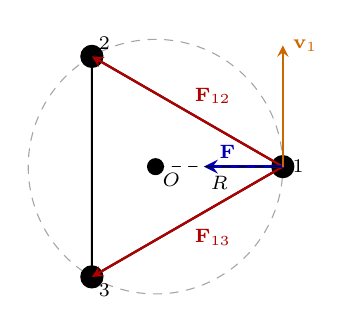
\begin{tikzpicture}[scale=2.8,>=stealth,line cap=round,line join=round]
  \coordinate (O) at (0,0);
  \coordinate (A) at (0.57735,0);
  \coordinate (B) at (-0.288675,0.5);
  \coordinate (C) at (-0.288675,-0.5);
  \draw[dashed,gray!70] (O) circle (0.57735);
  \draw[thick] (A)--(B)--(C)--cycle;
  \fill (O) circle (1.1pt) node[below right=-1pt,font=\scriptsize] {$O$};
  \fill (A) circle (1.5pt) node[right,font=\scriptsize] {$1$};
  \fill (B) circle (1.5pt) node[above right=-1pt,font=\scriptsize] {$2$};
  \fill (C) circle (1.5pt) node[below right=-1pt,font=\scriptsize] {$3$};
  \draw[->,red!70!black,thick] (A)--(B)
    node[midway,above right=-1pt,font=\scriptsize] {$\vect F_{12}$};
  \draw[->,red!70!black,thick] (A)--(C)
    node[midway,below right=-1pt,font=\scriptsize] {$\vect F_{13}$};
  \coordinate (P) at ($(A)!0.62!(O)$);
  \draw[->,blue!70!black,very thick] (A)--(P)
    node[midway,above left=-1pt,font=\scriptsize] {$\vect F$};
  \draw[->,orange!80!black,thick] (A)--++(0,0.55)
    node[right,font=\scriptsize] {$\vect v_1$};
  \draw[dashed] (O)--(A) node[midway,below,font=\scriptsize] {$R$};
\end{tikzpicture}
\caption{等边三角形构型的受力与速度示意（未按比例）。两引力夹角 $60^\circ$，合力指向中心。}
\label{fig:force}
\end{figure}

\subsection{解析轨道与有界性}
该模式的解析解为整个三角形以角速度 $\omega$ 刚性旋转：
\begin{equation}\label{eq:lagrange-exact}
\vect r_i(t)=R(\omega t)\vect r_i(0),
\qquad
\vect v_i(t)=R(\omega t)\vect v_i(0),
\end{equation}
其中 $R(\theta)$ 为逆时针旋转矩阵。因此三对距离严格恒为 1，最小距离和最大距离都为 1，
$0.05\le d_{ij}<10$ 对全部 $t$ 成立。图~\ref{fig:traj}(a) 用不同时刻的三角形快照显示这一
刚性旋转；图~\ref{fig:dist}(a) 的三条距离曲线重合为 $d=1$。从“有限时间有界”的判据看，
模式 A 是严格满足的。

\subsection{线性稳定性：周期不等于稳定}
在随三角形一起旋转的参考系中，Lagrange 构型是一个平衡点。设 $\boldsymbol\rho_i$ 为旋转系坐标，
线性化方程为
\begin{equation}\label{eq:lin}
\delta\ddot{\boldsymbol\rho}_i
=-\sum_j H_{ij}\delta\boldsymbol\rho_j
-2\omega J\,\delta\dot{\boldsymbol\rho}_i
+\omega^2\delta\boldsymbol\rho_i,
\qquad
J=\begin{pmatrix}0&-1\\1&0\end{pmatrix},
\end{equation}
其中 $H$ 是势能 $U=-\sum_{i<j}1/r_{ij}$ 的 Hessian。把 12 维线性系统写成矩阵并求特征值，
得到一对实部为正的复特征值
\begin{equation}\label{eq:eig}
\lambda=1.224745\pm1.732051\,\mathrm{i}.
\end{equation}
实部即最大增长率，e 折时间 $1/\lambda\approx0.816$。这意味着任何微小扰动都会以 $\ee^{\lambda t}$
增长：模式 A 虽严格周期，却是线性不稳定的。这一结论与“等边三角形解对等质量三体不稳定”的
经典结果一致。

\subsection{双精度能否模拟到 $t=50$？}
既然 $\lambda\approx1.2247$，初始误差 $\varepsilon$ 增长到 $O(1)$ 所需时间约为
$\ln(1/\varepsilon)/\lambda$。双精度舍入/截断误差约 $10^{-12}$--$10^{-16}$，对应
$t\approx20$--$30$；要在 $t=50$ 内保持 $O(1)$ 以下，需要
$\varepsilon<\ee^{-61}\approx10^{-27}$，即约 27 位十进制有效数字，普通双精度无法满足。
表~\ref{tab:precision} 给出了三组未扰动数值积分与解析解的偏差。

\begin{table}[H]
\centering\small
\caption{模式 A 未扰动数值积分与解析解的偏差}
\label{tab:precision}
\begin{tabular}{@{}lcccccc@{}}
\toprule
数值方案 & $t_{\rm end}$ & 停止原因 & $\max|\Delta E|/|E_0|$ & $t=20$ 偏差 & $t=30$ 偏差\\
\midrule
RK4, $\Delta t=0.002$ & 39.48 & 近距离 & $1.87\times10^{-4}$ & $2.07\times10^{-6}$ & $4.43\times10^{-1}$\\
RK4, $\Delta t=0.001$ & 50.00 & 完成 & $3.88\times10^{-6}$ & $2.07\times10^{-5}$ & $2.09$\\
DP45, $\mathrm{rtol}=10^{-13}$ & 40.98 & 近距离 & $3.07\times10^{-12}$ & $1.98\times10^{-6}$ & $4.05\times10^{-1}$\\
\bottomrule
\end{tabular}
\end{table}

可以看到：三种方案的偏差都在 $t\approx20$ 后迅速增大，$t=30$ 时已到 $O(0.4$--$2)$。
RK4 $\Delta t=0.001$ 恰好在 $t=50$ 前没有触发 $0.05$ 预警（$d_{\min}=0.064$），
但它在 $t=30$ 时已偏离解析解 $2.09$，轨迹早已不是原来的旋转三角形。这说明“没有触发预警”
不能证明模拟正确；能量误差也只有 $3.9\times10^{-6}$，同样不能保证轨迹精度。

因此，\textbf{模式 A 的轨迹、距离和有界性数据采用解析解}；数值积分只用于研究不稳定性和
数值精度，不用于声称“数值上模拟了 50 时间的三角形”。图~\ref{fig:sep}(b) 把数值误差包络与
$10^{-4}$ 的物理扰动画在一起：两者斜率都接近 $\ee^{1.2247t}$，只是起点不同
（数值误差 $10^{-12}$--$10^{-6}$，物理扰动 $10^{-4}$）。这正是“同一不稳定模式被不同初始误差
触发”的直接证据。

% ================= 4 模式 B =================
\section{模式 B：8 字形运动}\label{sec:eight}

题目给出的 8 字形初值为
\begin{gather}
\vect r_1=(0.97000436,-0.24308753),\qquad
\vect r_2=-\vect r_1,\qquad
\vect r_3=\vect 0,\label{eq:icB-r}\\
\vect v_1=\vect v_2=(0.46620369,0.43236573),\qquad
\vect v_3=-2\vect v_1.\label{eq:icB-v}
\end{gather}
这组初值经过四舍五入，严格说只是近似周期轨道；文献中的周期为 $T\approx6.3259$。
直接积分得 $E_0=-1.287142$、$L=0$（机器精度），在 $0\le t\le50$ 内（约 7.9 个周期）
$d_{\min}=0.6905$、$d_{\max}=2.0000$，未触发 $0.05$ 预警，也未逃逸。
图~\ref{fig:traj}(b) 显示三颗星共用同一条 8 字曲线，只是相位不同；
图~\ref{fig:dist}(b) 显示三对距离在 $0.69$--$2.0$ 之间周期振荡。

8 字形的运动结构是“舞蹈型”（choreography）：三颗星依次沿同一条闭合曲线运动，在任意时刻
它们位于曲线的不同段上。它与模式 A 的刚性三角形有本质区别：A 是三体保持固定形状整体旋转，
B 是三体沿同一条轨道追逐，形状不断变化。

已有理论结果表明，等质量 8 字形轨道是线性稳定的（Sim\'o 等）。本文的扰动实验（\S\ref{sec:pert}）
与之相符：$10^{-4}$ 的扰动只产生 $6.3\times10^{-3}$ 的分离，50 时间内没有失稳。但要注意，
给定初值只有 8 位有效数字，实际数值轨道是严格周期轨道附近的准周期轨道；50 时间内的有界性
不能外推为永久稳定。

% ================= 5 其他模式 =================
\section{其他有界模式：飞蛾 I 与层级三体}\label{sec:others}

\subsection{搜索策略与候选筛选}
为了寻找题目要求的新模式，本文采用两类策略。第一类是零角动量对称族：取
$\vect r_1=(-1,0)$、$\vect r_2=(1,0)$、$\vect r_3=\vect0$，
$\vect v_1=\vect v_2=(v_x,v_y)$、$\vect v_3=-2\vect v_1$，
这样质心在原点、总动量为零、总角动量为零。Šuvakov 与 Dmitrašinović 在这一族中给出了一批
平面周期轨道（butterfly、moth、goggles、yarn、yin-yang 等），其初值和周期可查。本文把这些
初值当作候选，用自己的积分器独立检验，而不是直接相信文献。

筛选标准严格按题意：在 $0\le t\le50$ 内（周期短于 50 的积分一个周期）
$d_{\min}\ge0.05$ 且 $d_{\max}<10$。图~\ref{fig:screening} 把所有候选画在
$(d_{\min},d_{\max})$ 平面上；表~\ref{tab:screening} 列出具体数值。结果非常清楚：
\textbf{15 个已发表候选里只有 moth I（飞蛾 I）通过}，其余的最小距离都远小于 $0.05$
（butterfly I 为 $0.0110$，butterfly II 为 $0.0041$，goggles 为 $0.0185$，yarn 为 $0.0050$，
butterfly IV 甚至只有 $2.9\times10^{-5}$）。这些轨道在数学上是漂亮周期解，但在题目给定的
$0.05$ 阈值下不合格。

需要说明：如果把某个紧致轨道整体放大，$d_{\min}$ 会随之增大，可能满足 $0.05$；但题目明确
规定“仅对同一轨道做尺度变换不算找到新模式”，所以本文不把缩放后的同一轨道当作新模式。
本文保留的第二个新模式是自行构造的层级三体，它与对称族的舞蹈型轨道在运动结构上完全不同。

\begin{table}[H]
\centering\footnotesize
\setlength{\tabcolsep}{3.6pt}
\caption{已发表对称族候选轨道的筛选（周期短于 50 的积分一个周期，否则积分到 $t=50$）}
\label{tab:screening}
\begin{tabular}{@{}lcccccc@{}}
\toprule
候选 & $v_x$ & $v_y$ & $T$ & $d_{\min}$ & $d_{\max}$ & 有效？\\
\midrule
butterfly I  & 0.30689 & 0.12551 & 6.2356  & $1.102\times10^{-2}$ & 2.0000 & 否\\
butterfly II & 0.39295 & 0.09758 & 7.0039  & $4.099\times10^{-3}$ & 2.0000 & 否\\
bumblebee    & 0.18428 & 0.58719 & 63.5345 & $1.191\times10^{-2}$ & 2.1667 & 否\\
moth I       & 0.46444 & 0.39606 & 14.8939 & $7.945\times10^{-2}$ & 2.1601 & \textbf{是}\\
moth II      & 0.43917 & 0.45297 & 28.6703 & $4.967\times10^{-2}$ & 2.2553 & 否\\
butterfly III& 0.40592 & 0.23016 & 13.8658 & $8.335\times10^{-3}$ & 2.0000 & 否\\
moth III     & 0.38344 & 0.37736 & 25.8406 & $6.714\times10^{-3}$ & 2.0000 & 否\\
goggles      & 0.08330 & 0.12789 & 10.4668 & $1.848\times10^{-2}$ & 2.0930 & 否\\
butterfly IV & 0.350112& 0.07934 & 79.4759 & $2.875\times10^{-5}$ & 2.0000 & 否\\
dragonfly    & 0.08058 & 0.58884 & 21.2710 & $7.332\times10^{-3}$ & 2.0250 & 否\\
yarn         & 0.55906 & 0.34919 & 55.5018 & $4.977\times10^{-3}$ & 2.7722 & 否\\
yin-yang I a & 0.51394 & 0.30474 & 17.3284 & $1.327\times10^{-2}$ & 2.7138 & 否\\
yin-yang I b & 0.28270 & 0.32721 & 10.9626 & $9.784\times10^{-3}$ & 2.0000 & 否\\
yin-yang II a& 0.41682 & 0.33033 & 55.7898 & $1.948\times10^{-4}$ & 2.0387 & 否\\
yin-yang II b& 0.41734 & 0.31310 & 54.2076 & $1.912\times10^{-4}$ & 2.0000 & 否\\
\bottomrule
\end{tabular}
\end{table}

\begin{figure}[H]
\centering
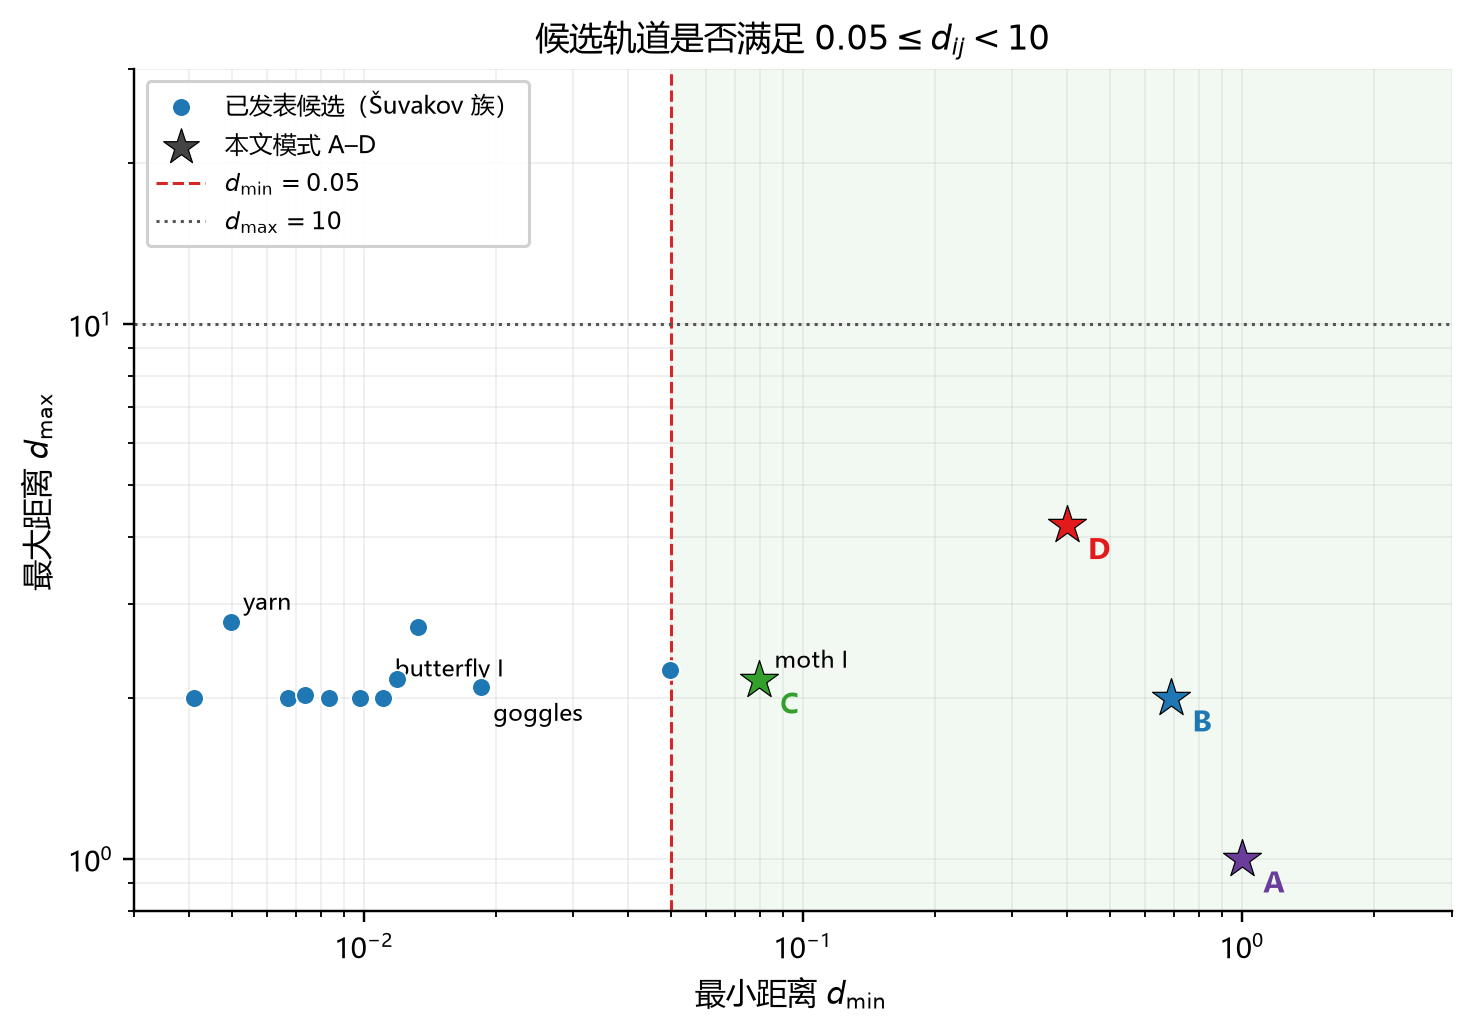
\includegraphics[width=0.72\textwidth]{fig7_screening.png}
\caption{候选轨道的 $(d_{\min},d_{\max})$ 分布。绿色区域为 $0.05\le d_{\min}$ 且 $d_{\max}<10$；
只有 moth I 落在区域内，A--D 为本文四种模式。}
\label{fig:screening}
\end{figure}

\subsection{模式 C：飞蛾 I（moth I）}
飞蛾 I 的初值为 $\vect r_1=(-1,0)$、$\vect r_2=(1,0)$、$\vect r_3=\vect0$，
$\vect v_1=\vect v_2=(0.46444,0.39606)$、$\vect v_3=(-0.92888,-0.79212)$。文献周期
$T\approx14.8939$。直接积分得 $E_0=-1.382296$、$L=0$；在 $0\le t\le50$ 内
$d_{\min}=0.0794$、$d_{\max}=2.1601$，未触发预警。图~\ref{fig:traj}(c) 是它的轨迹：
三条曲线相互穿插，形成一个类似飞蛾翅膀的图案，与 8 字形的单一闭合曲线明显不同；
图~\ref{fig:dist}(c) 显示 $d_{13}/d_{23}$ 会周期性地下探到 $0.08$ 左右，最近一次出现在
$t\approx24.6$，之后在 $t\approx47$ 附近还有一次。

飞蛾 I 的最小距离只比 $0.05$ 大 $0.029$，属于“边缘合格”。这不是一个很安全的模式：
任何额外的扰动或数值误差都可能把某次交会推到阈值以下。后文的扰动实验会看到，$10^{-4}$ 的
扰动虽然没有触发预警，但分离可达 $1.2\times10^{-2}$，最小距离降到 $0.0793$，已经非常接近边界。

\subsection{模式 D：层级三体（紧密双星 + 远方第三体）}
第二个新模式由两个时间尺度相差很大的子系统组成：恒星 1、2 组成间距 $d=0.4$ 的紧密圆双星，
恒星 3 在半径约 $2.67$ 的宽轨道上绕整个系统的质心运动。构造如下。双星内部每颗星到双星质心
的距离为 $d/2$，圆运动速度为
\begin{equation}\label{eq:vint}
v_{\rm int}=\sqrt{\frac{1}{2d}}=\sqrt{1.25}\approx1.118034.
\end{equation}
把双星看成一个总质量 2 的质点，它与星 3 的相对圆轨道半径取 $R=4$，相对速度为
\begin{equation}\label{eq:vrel}
v_{\rm rel}=\sqrt{\frac{3}{R}}=\sqrt{0.75}\approx0.866025.
\end{equation}
为保证质心静止，双星质心位于 $-R/3$、星 3 位于 $2R/3$；速度按质量反比分配：双星质心速度
$-v_{\rm rel}/3$，星 3 速度 $2v_{\rm rel}/3$。把双星内部速度叠加到 1、2 号星上，得到
\begin{align}
\vect r_1&=(-1.533333,0),&
\vect r_2&=(-1.133333,0),&
\vect r_3&=(2.666667,0),\label{eq:icD-r}\\
\vect v_1&=(0,0.829359),&
\vect v_2&=(0,-1.406709),&
\vect v_3&=(0,0.577350).\label{eq:icD-v}
\end{align}
代入得 $E_0\approx-1.501253$、$L\approx1.862187$，质心位置和速度均为零（数值上到 $10^{-16}$）。
该构型的时间尺度为：双星内部周期 $T_{\rm in}=\pi d/v_{\rm int}\approx1.12$，外层轨道周期
$T_{\rm out}=2\pi R/v_{\rm rel}\approx29.0$，两者相差约 26 倍。双星的 Hill 半径约为
$R(2/3)^{1/3}\approx3.5$，远大于 $d=0.4$，所以第三体不会轻易撕开双星。

数值积分到 $t=50$ 得 $d_{\min}=0.3993$、$d_{\max}=4.2000$，未触发预警，也未逃逸。
图~\ref{fig:traj}(d) 显示双星的两个小环在一个大圆内运动，插图是 1--2 的相对轨道；
图~\ref{fig:dist}(d) 显示双星间距在 $0.399$--$0.401$ 之间小幅振荡（第三体的潮汐扰动），
而 $d_{13}/d_{23}$ 在 $3.78$--$4.20$ 之间变化。

模式 D 的运动结构与 A、B、C 都不同：它不是三体对称的舞蹈型轨道，而是“双星 + 第三体”的
层级结构，两个子系统的时间尺度分离是它保持有界的主要原因。它也不是严格周期轨道，但在 50
时间内表现出很好的规则性和鲁棒性。

\subsection{模式汇总与结构比较}
四种模式的结构差异可以概括为：\textbf{A} 是三体保持等边形状的整体刚性旋转，三对距离恒定；
\textbf{B} 是三体沿同一条 8 字曲线依次追逐的舞蹈型轨道，零角动量；\textbf{C} 是同一对称族中
另一种舞蹈型轨道，轨迹呈飞蛾状、有更近的双星式交会，周期和最小距离都不同；\textbf{D} 是层级
结构，一个紧密双星加一个远距离第三体，两个时间尺度分离。它们不是彼此的整体旋转、平移、
速度方向旋转或尺度变换，因此按题目规则应计为不同模式。

\begin{table}[H]
\centering\small
\caption{四种有界模式的汇总（$0\le t\le50$；模式 A 为解析解）}
\label{tab:modes}
\begin{tabular}{@{}clcccccc@{}}
\toprule
模式 & 名称 & $t_{\rm end}$ & 提前停止 & $d_{\min}$ & $d_{\max}$ & $E_0$ & $\max|\Delta E|/|E_0|$\\
\midrule
A & Lagrange 三角形 & 50（解析） & 否 & 1.0000 & 1.0000 & $-1.500000$ & 0\\
B & 8 字形 & 50.00 & 否 & 0.6905 & 2.0000 & $-1.287142$ & $1.81\times10^{-12}$\\
C & 飞蛾 I & 50.00 & 否 & 0.0794 & 2.1601 & $-1.382296$ & $7.94\times10^{-12}$\\
D & 层级三体 & 50.00 & 否 & 0.3993 & 4.2000 & $-1.501253$ & $1.54\times10^{-11}$\\
\bottomrule
\end{tabular}
\end{table}

\begin{table}[H]
\centering\footnotesize
\setlength{\tabcolsep}{3pt}
\caption{四种模式的完整初始条件（$G=m=1$；质心在原点，总动量为零）}
\label{tab:ic}
\begin{tabular}{@{}lcccc@{}}
\toprule
 & A & B & C & D\\
\midrule
$\vect r_1$ & \makecell{$(0.577350,$\\$0.000000)$} & \makecell{$(0.970004,$\\$-0.243088)$} & \makecell{$(-1.000000,$\\$0.000000)$} & \makecell{$(-1.533333,$\\$0.000000)$}\\
$\vect r_2$ & \makecell{$(-0.288675,$\\$0.500000)$} & \makecell{$(-0.970004,$\\$0.243088)$} & \makecell{$(1.000000,$\\$0.000000)$} & \makecell{$(-1.133333,$\\$0.000000)$}\\
$\vect r_3$ & \makecell{$(-0.288675,$\\$-0.500000)$} & \makecell{$(0.000000,$\\$0.000000)$} & \makecell{$(0.000000,$\\$0.000000)$} & \makecell{$(2.666667,$\\$0.000000)$}\\
$\vect v_1$ & \makecell{$(0.000000,$\\$1.732051)$} & \makecell{$(0.466204,$\\$0.432366)$} & \makecell{$(0.464440,$\\$0.396060)$} & \makecell{$(0.000000,$\\$0.829359)$}\\
$\vect v_2$ & \makecell{$(-0.866025,$\\$-0.500000)$} & \makecell{$(0.466204,$\\$0.432366)$} & \makecell{$(0.464440,$\\$0.396060)$} & \makecell{$(0.000000,$\\$-1.406709)$}\\
$\vect v_3$ & \makecell{$(0.866025,$\\$-0.500000)$} & \makecell{$(-0.932407,$\\$-0.864731)$} & \makecell{$(-0.928880,$\\$-0.792120)$} & \makecell{$(0.000000,$\\$0.577350)$}\\
\bottomrule
\end{tabular}
\end{table}

\begin{figure}[H]
\centering
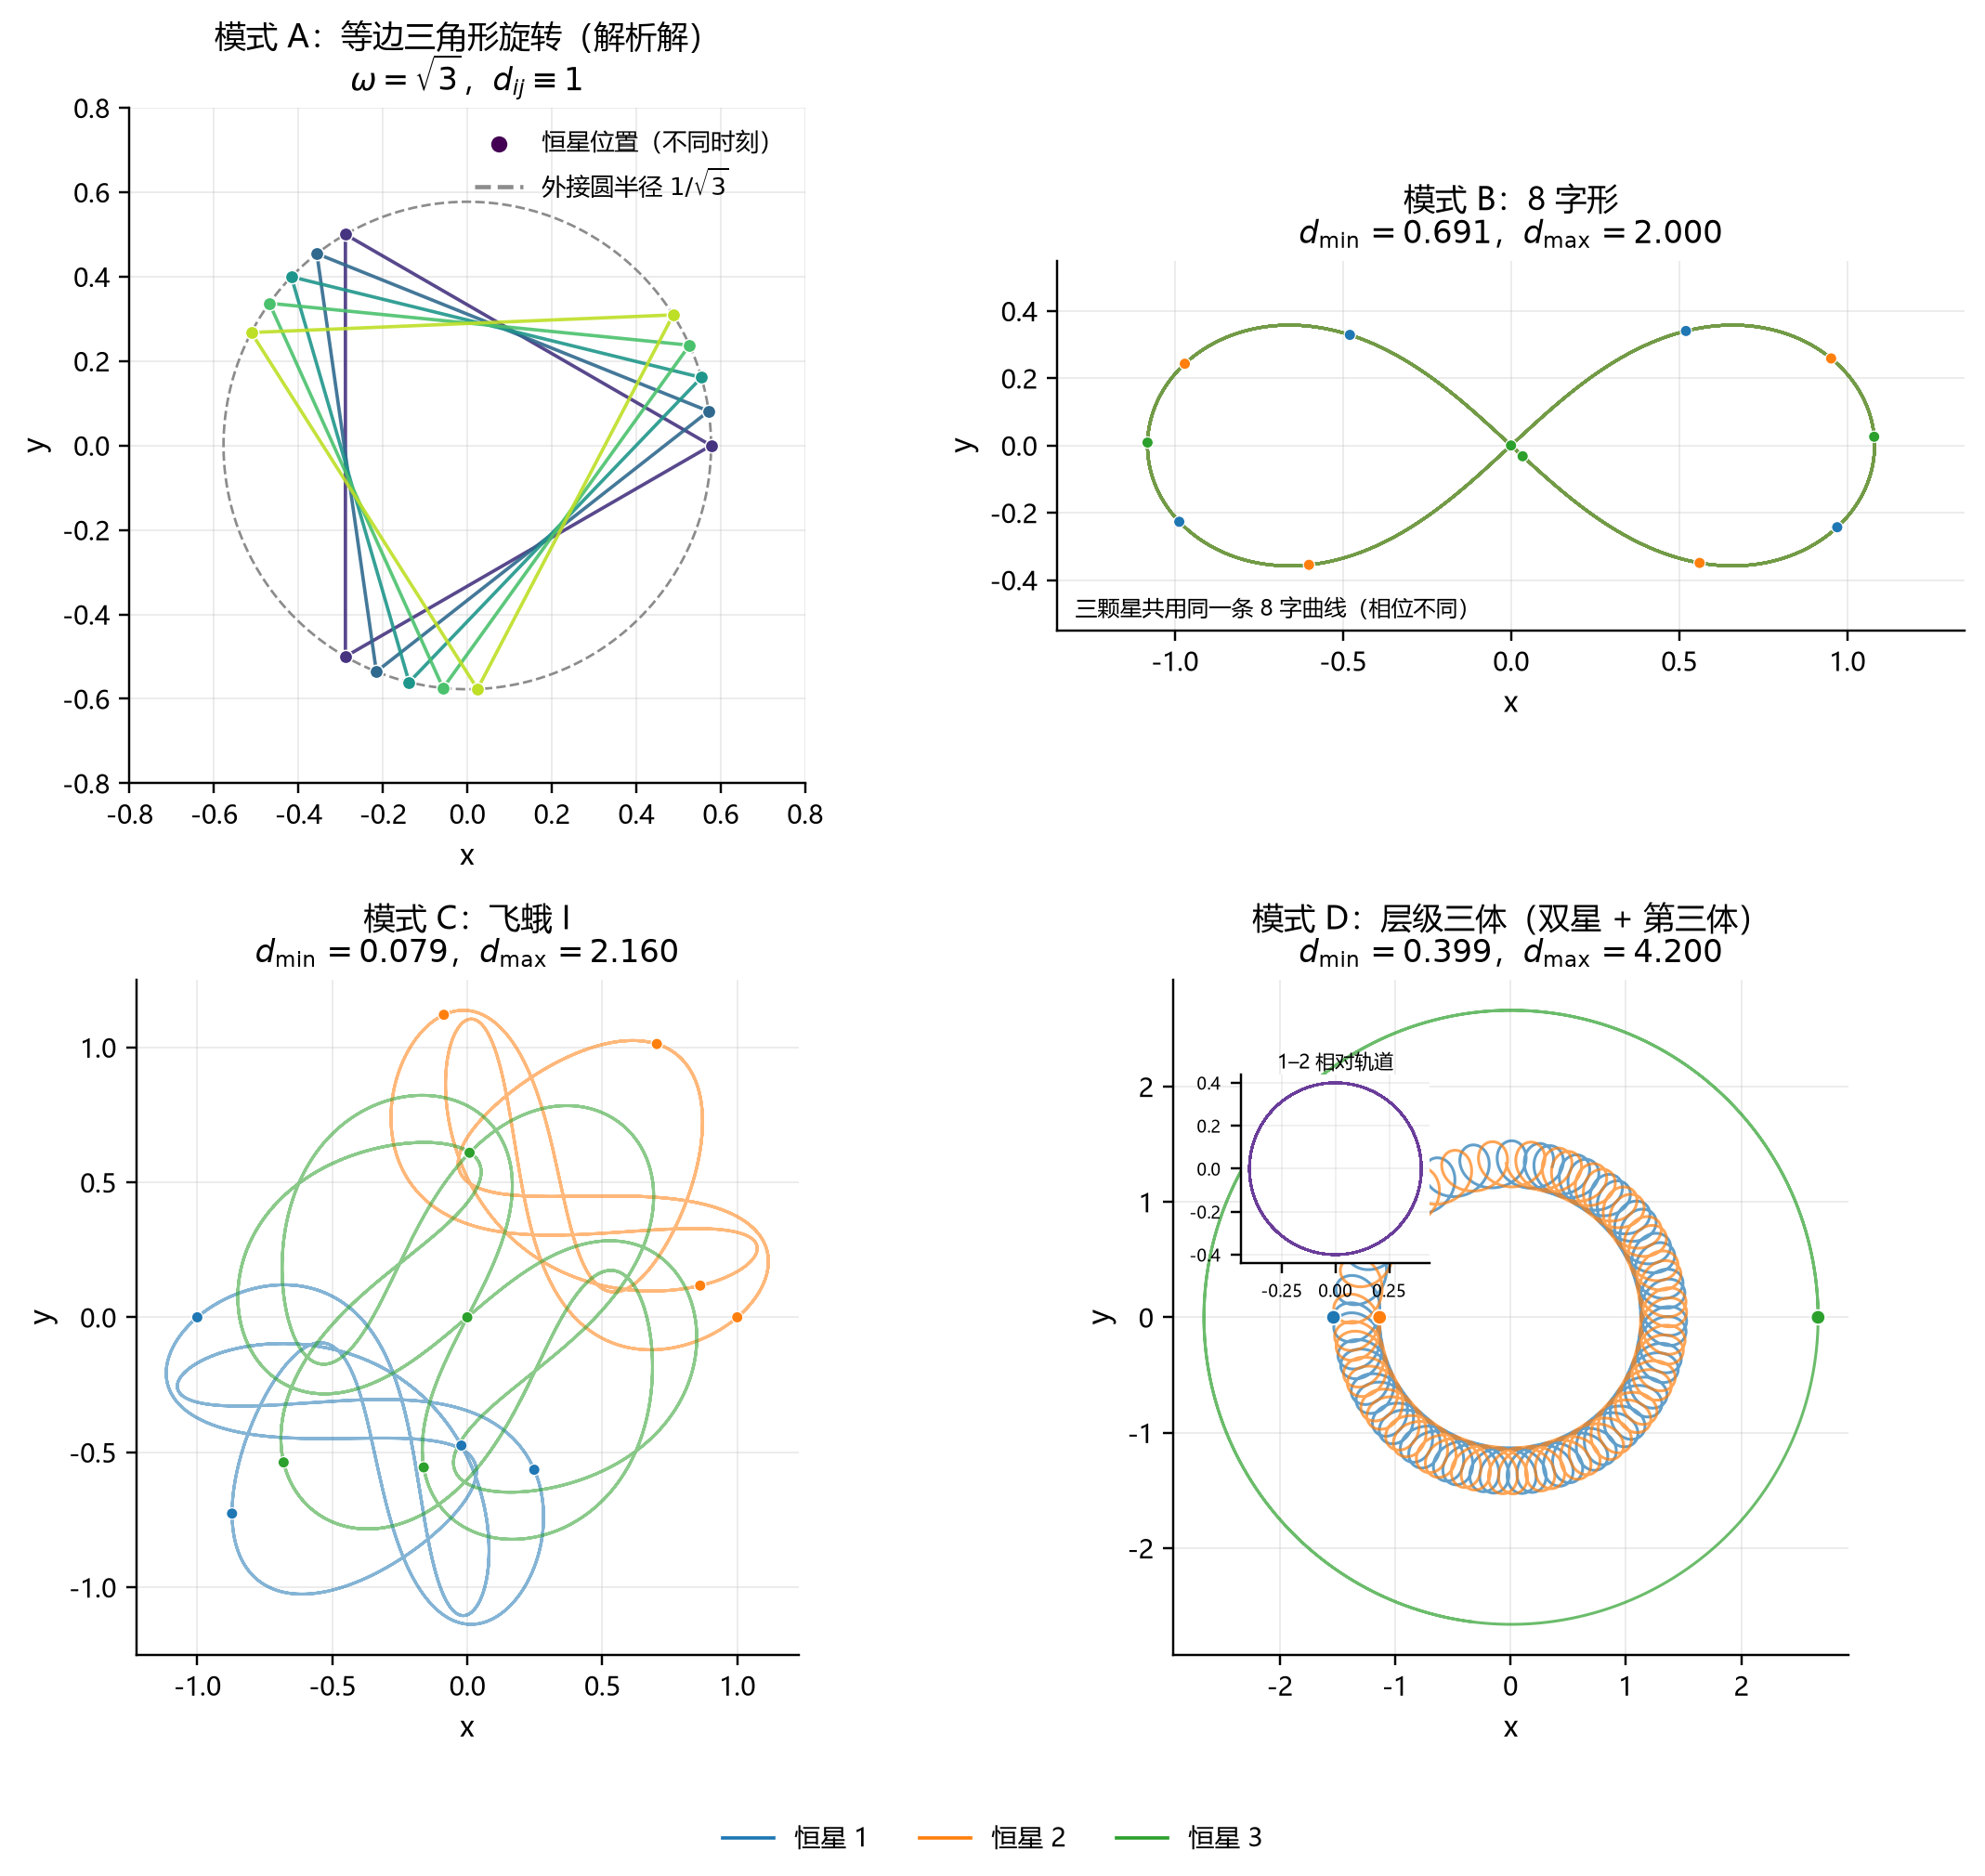
\includegraphics[width=0.92\textwidth]{fig1_trajectories.png}
\caption{四种模式的轨迹。(a) 等边三角形：不同时刻的三角形快照；(b) 8 字形：三颗星共用同一条
曲线；(c) 飞蛾 I；(d) 层级三体，插图为 1--2 的相对轨道。}
\label{fig:traj}
\end{figure}

图~\ref{fig:traj} 中的轨迹只反映几何形状；图~\ref{fig:dist} 进一步给出三对距离的定量信息。
A 的 $d_{12}=d_{13}=d_{23}=1$，说明三角形在旋转过程中不变形；B 的三条曲线在 $0.69$--$2.0$
之间振荡，说明三体沿同一条 8 字曲线以不同相位追逐；C 的 $d_{13}/d_{23}$ 会下探到 $0.079$，
这是它“边缘”的原因；D 的双星间距几乎不变（$0.399$--$0.401$），第三体距离在 $3.78$--$4.20$
之间，体现层级结构。表~\ref{tab:ic} 给出了全部初值，读者可据此复现。后文的扰动实验将围绕
这些距离特征展开。

\begin{figure}[H]
\centering
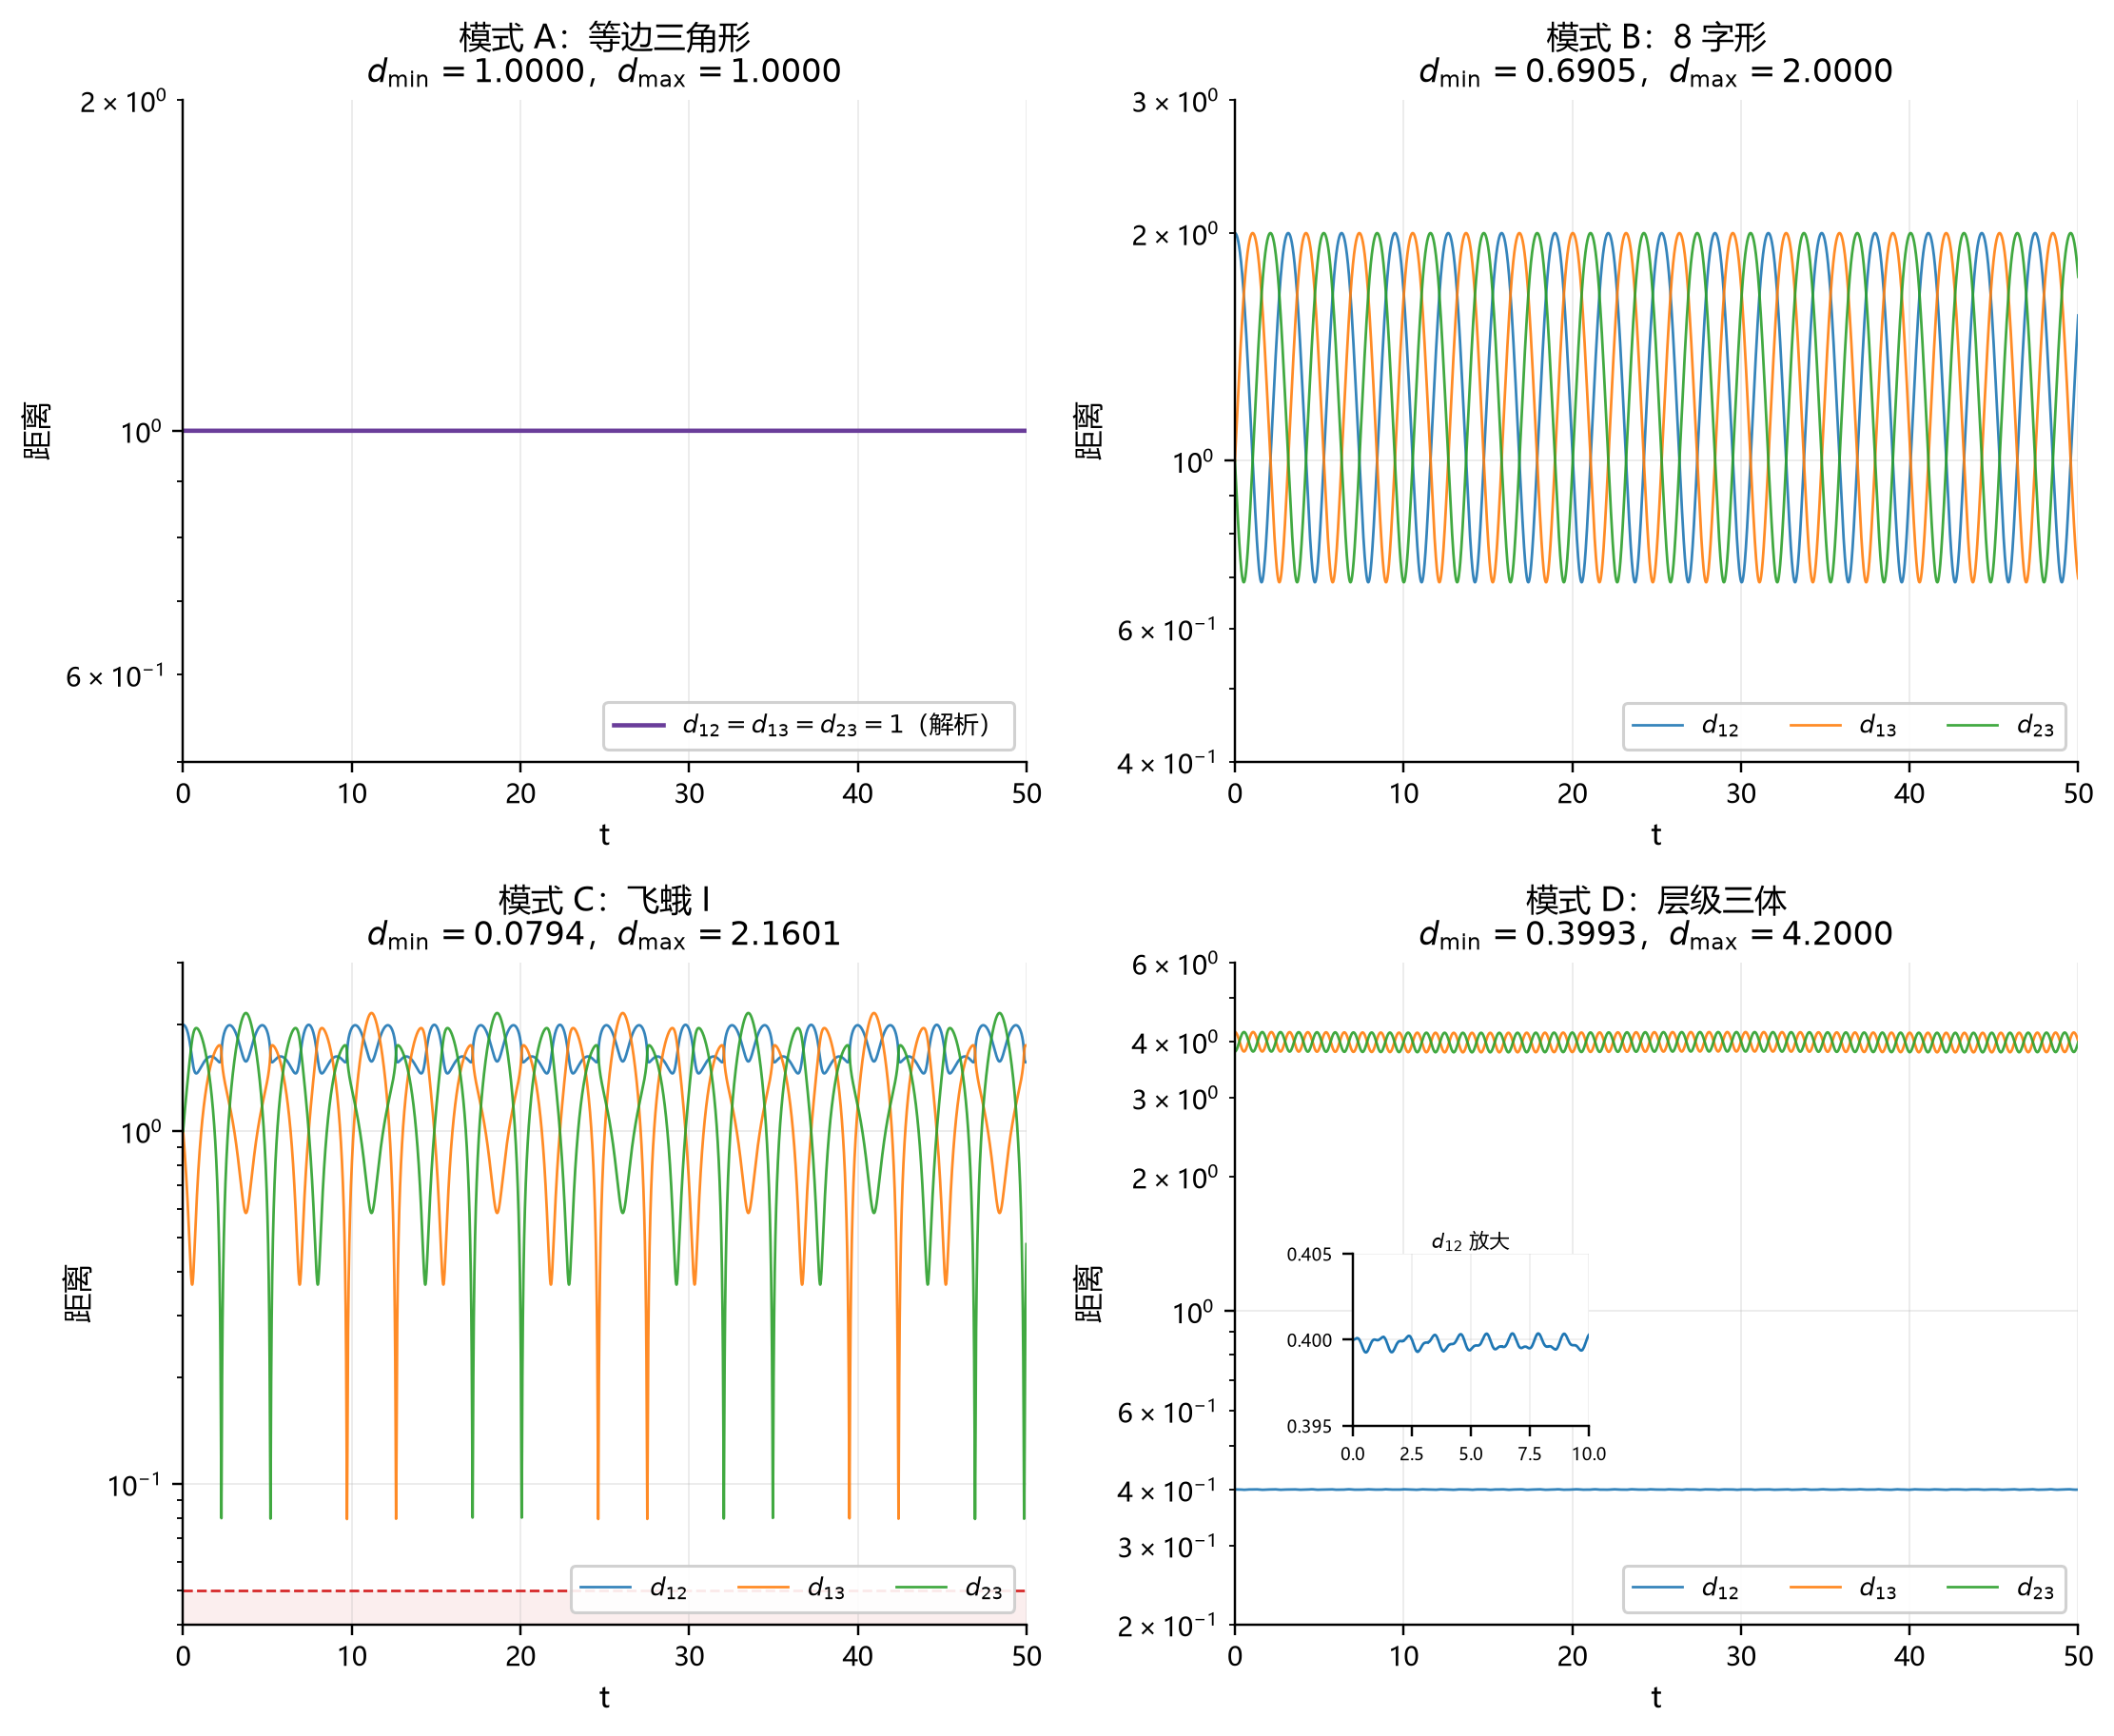
\includegraphics[width=0.92\textwidth]{fig2_distances.png}
\caption{四种模式的恒星间距离。红虚线为 $0.05$ 预警阈值，灰色点线为 10 的上界；纵轴为对数坐标。}
\label{fig:dist}
\end{figure}

% ================= 6 扰动实验 =================
\section{扰动实验：有限时间有界 \texorpdfstring{$\ne$}{≠} 对扰动稳定}\label{sec:pert}

\subsection{扰动方案}
按题目要求，对每个模式把恒星 1 的初始 $v_x$ 增加 $10^{-4}$，然后统一减去三颗星的质心速度，
使总动量重新为零。被扰动的初始速度为
\begin{equation}\label{eq:pert}
\vect v_1\leftarrow\vect v_1+(10^{-4},0),
\qquad
\vect v_i\leftarrow\vect v_i-\vect V_{\rm cm}\quad(i=1,2,3).
\end{equation}
扰动后的轨道与未扰动轨道用同一高精度积分器计算（DP45，$\mathrm{rtol}=10^{-13}$）。
模式 A 的未扰动参考用解析解；B、C、D 用各自的未扰动数值轨道。为隔离数值误差，扰动实验
不使用 RK4 $\Delta t=0.002$；\S\ref{sec:step} 会说明原因。

\subsection{结果}
\begin{table}[H]
\centering\footnotesize
\setlength{\tabcolsep}{4pt}
\caption{$10^{-4}$ 速度扰动前后的最小/最大距离与末端分离}
\label{tab:pert}
\begin{tabular}{@{}lccccccc@{}}
\toprule
模式 & $d_{\min}$（未） & $d_{\min}$（扰） & $d_{\max}$（未） & $d_{\max}$（扰） & $\delta_{\rm end}$ & $t_{\rm end}$/停止 & 判定\\
\midrule
A & 1.0000 & 0.0499 & 1.0000 & 2.4711 & $9.99\times10^{-1}$ & 15.55/近距离 & 指数失稳\\
B & 0.6905 & 0.6904 & 2.0000 & 2.0002 & $6.32\times10^{-3}$ & 50.00/完成 & 有界，缓慢分离\\
C & 0.0794 & 0.0793 & 2.1601 & 2.1602 & $4.76\times10^{-3}$ & 50.00/完成 & 有界，边缘\\
D & 0.3993 & 0.3993 & 4.2000 & 4.2000 & $4.73\times10^{-4}$ & 50.00/完成 & 有界，鲁棒\\
\bottomrule
\end{tabular}
\end{table}

\begin{figure}[H]
\centering
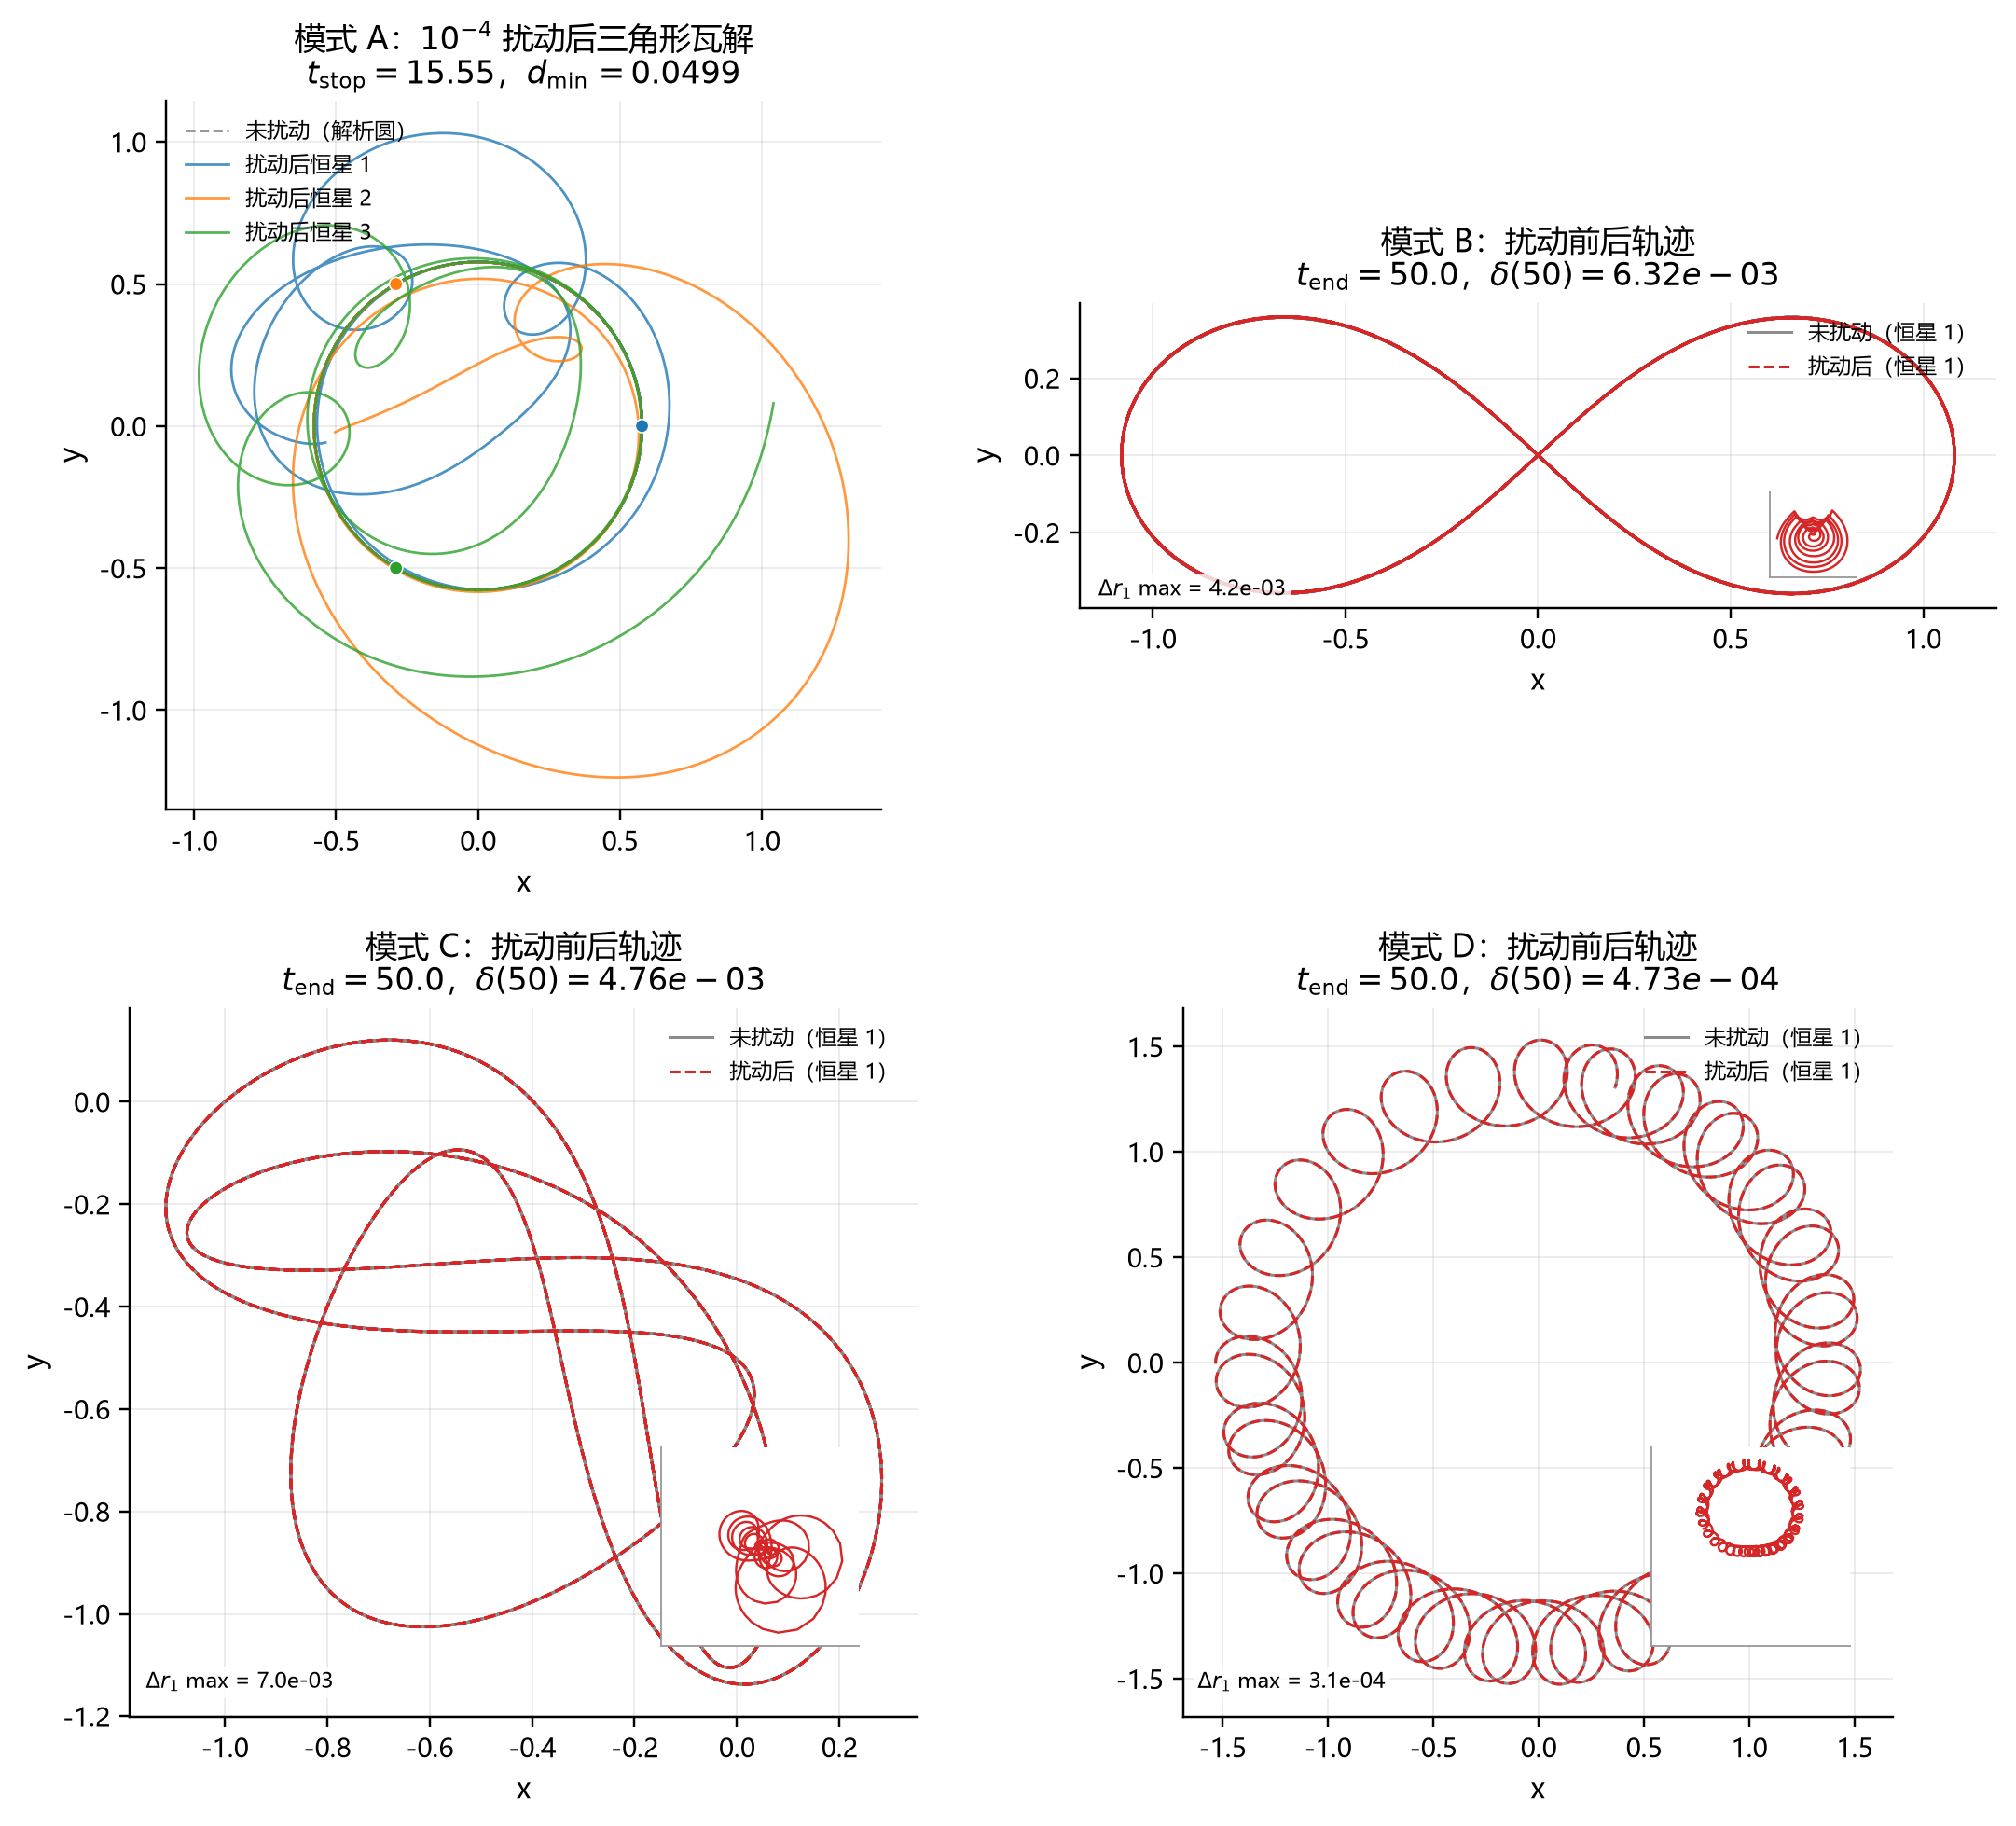
\includegraphics[width=0.92\textwidth]{fig3_perturbation.png}
\caption{扰动前后的轨迹对比。灰色为未扰动，红色为扰动后；B、C、D 的插图为恒星 1 的扰动位移
$\Delta\vect r_1$。}
\label{fig:pert}
\end{figure}

\textbf{模式 A：} $\delta(t)$ 从 $10^{-4}$ 开始，以接近 $\ee^{1.2247t}$ 的斜率增长，
$t\approx8$ 时达到 $O(1)$，三角形已经瓦解；$t=15.55$ 时某两颗星的距离降到 $0.05$ 以下，
计算停止（$d_{\min}=0.0499$，$d_{\max}=2.47$）。对 $\delta(t)$ 在 $t=1$--$6$ 做指数拟合得
$\lambda\approx1.17$，略低于线性值 $1.2247$；这是因为初始扰动包含多个本征模式，且后期出现
非线性饱和。图~\ref{fig:sep}(a) 中紫色曲线与黑色虚线（拟合）几乎重合。这个结果说明：
模式 A 的“周期”只在精确的数学解中存在，任何 $10^{-4}$ 的扰动都会在十几个时间单位内摧毁它。

\textbf{模式 B：} 扰动后 $\delta$ 缓慢增长到 $6.3\times10^{-3}$，$d_{\min}$ 从 $0.69053$ 降到
$0.69036$，$d_{\max}$ 从 $2.0$ 增到 $2.00019$，50 时间内没有触发预警。$\delta$ 的增长远慢于
指数（拟合 $\lambda\approx0.26$，且不是直线），与 8 字形已知的线性稳定性一致。但“50 时间内
有界”仍不是永久稳定的证明；更严格的结论需要 Floquet 分析或长期积分。

\textbf{模式 C：} 扰动后 $\delta$ 最大 $1.19\times10^{-2}$，末端 $4.76\times10^{-3}$；
$d_{\min}$ 从 $0.07940$ 降到 $0.07933$，$d_{\max}$ 从 $2.16006$ 增到 $2.16018$，
仍未触发预警。它是有界的，但最小距离只比阈值大 $0.029$，扰动已经把某次交会推得更近；
这是一个“边缘稳定”的案例，不能据此声称长期稳定。

\textbf{模式 D：} 扰动后 $\delta$ 最大 $7.6\times10^{-4}$，末端 $4.7\times10^{-4}$；
$d_{\min}$、$d_{\max}$ 在四位小数内几乎不变。双星的内部运动很快（周期 1.12），第三体的
外轨道很慢（周期 29），扰动主要在双星内部相位上，不会立即破坏层级结构。这是四种模式中对
$10^{-4}$ 扰动最鲁棒的一个。

\begin{figure}[H]
\centering
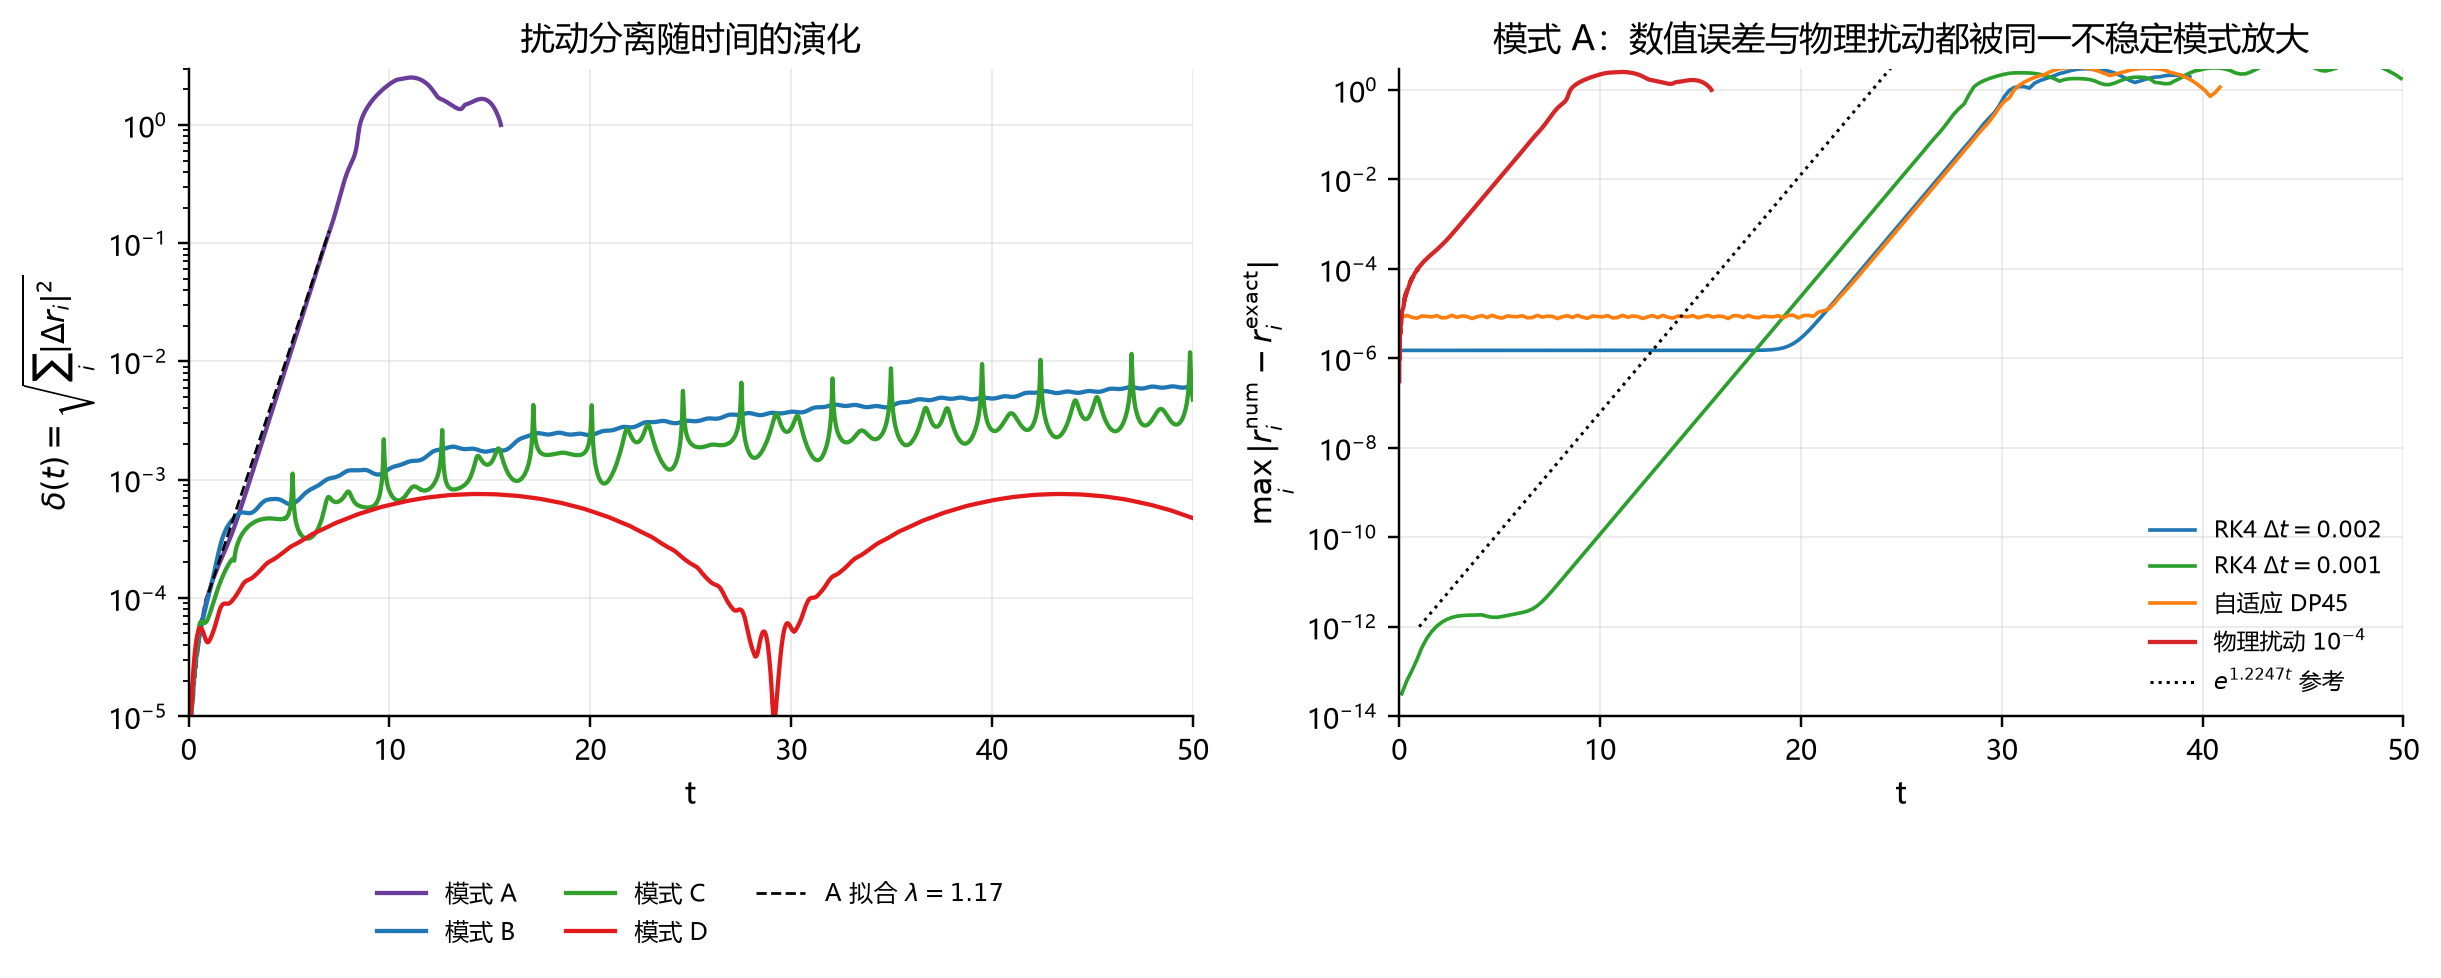
\includegraphics[width=0.95\textwidth]{fig4_separation.png}
\caption{(a) 四种模式的扰动分离 $\delta(t)$；(b) 模式 A 的数值误差包络与 $10^{-4}$ 物理扰动
对比，黑点线为 $\ee^{1.2247t}$ 参考。}
\label{fig:sep}
\end{figure}

\subsection{如何理解“稳定”}
把四个结果放在一起，可以得到三个层次的区别：
\begin{itemize}[leftmargin=2em,itemsep=2pt]
\item \textbf{有限时间有界}：只要求 $0\le t\le50$ 内 $0.05\le d_{ij}<10$。四种模式都满足
（A 由解析解，B/C/D 由数值积分）。
\item \textbf{对扰动有界（Lyapunov 意义下的有限时间稳定）}：给 $10^{-4}$ 扰动后仍不触发预警、
仍保持有界。B、C、D 满足；A 不满足。
\item \textbf{永久稳定}：对所有时间、所有足够小的扰动都有界。本文没有证明任何一种模式永久稳定；
B 有已知的线性稳定性结果，C、D 只有 50 时间的数值证据。
\end{itemize}
因此，题目中“在 $t\le50$ 内没有失稳不等于永久稳定；未扰动轨道周期重复，也不自动意味着对
扰动稳定”在模式 A 上体现得最清楚：它是严格周期解，却指数不稳定；而模式 B 的周期轨道在 50
时间内对扰动有界，但也不能仅凭这一点断言永久稳定。

% ================= 7 步长与能量 =================
\section{步长、能量误差与数值局限}\label{sec:step}

\subsection{实验设置}
对 8 字形和飞蛾 I，用固定步长 RK4 分别取 $\Delta t=0.002,0.001,0.0005$，积分到 $t=50$。
定义相对能量误差
\begin{equation}\label{eq:ee}
\varepsilon_E(t)=\frac{|E(t)-E(0)|}{|E(0)|},
\end{equation}
记录全程最大值；同时记录 $d_{\min}$、$d_{\max}$，并以 $\Delta t=0.002$ 的严格相同时间网格
为基准，比较位置、速度和最小距离的差异（不做插值）。

\begin{table}[H]
\centering\scriptsize
\setlength{\tabcolsep}{2.8pt}
\caption{RK4 步长对能量误差和距离的影响（差异均相对 $\Delta t=0.002$）}
\label{tab:step}
\begin{tabular}{@{}lccccccccc@{}}
\toprule
模式 & $\Delta t$ & $\max\varepsilon_E$ & 误差比 & 观测阶 $p$ & $d_{\min}$ & $d_{\max}$ & 最大位置差 & 最大 $d_{\min}$ 差\\
\midrule
B & 0.002  & $6.64\times10^{-12}$ & 33.8 & 5.08 & 0.690527 & 2.000000 & --- & ---\\
B & 0.001  & $1.97\times10^{-13}$ & 6.26 & 2.65 & 0.690527 & 2.000000 & $1.22\times10^{-9}$ & $7.63\times10^{-10}$\\
B & 0.0005 & $3.14\times10^{-14}$ & --- & --- & 0.690527 & 2.000000 & $1.32\times10^{-9}$ & $8.03\times10^{-10}$\\
C & 0.002  & $2.46\times10^{-4}$ & 31.8 & 4.99 & 0.079388 & 2.159999 & --- & ---\\
C & 0.001  & $7.72\times10^{-6}$ & 31.9 & 5.00 & 0.079422 & 2.160056 & $4.19\times10^{-2}$ & $2.95\times10^{-2}$\\
C & 0.0005 & $2.42\times10^{-7}$ & --- & --- & 0.079405 & 2.160061 & $4.32\times10^{-2}$ & $3.04\times10^{-2}$\\
\bottomrule
\end{tabular}
\end{table}

\begin{figure}[H]
\centering
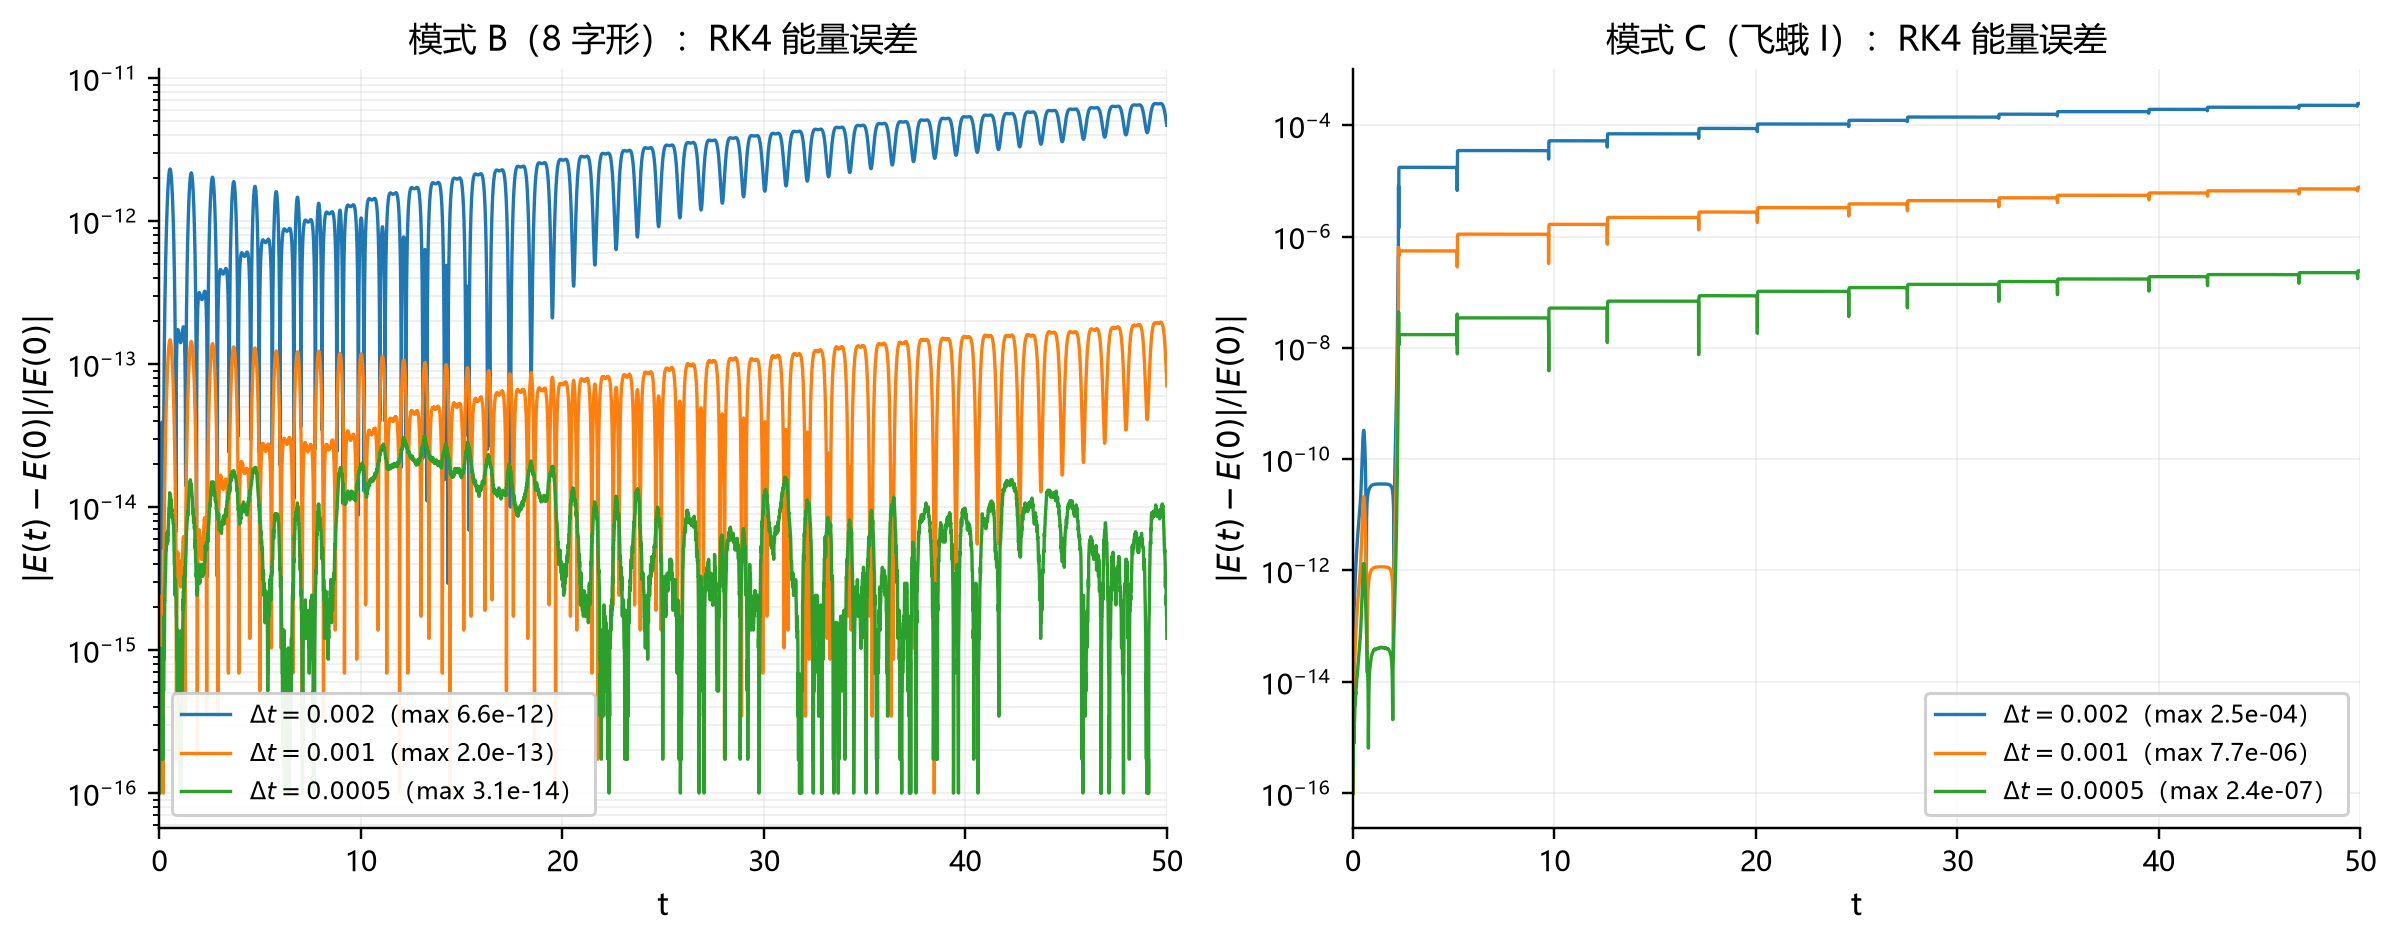
\includegraphics[width=0.95\textwidth]{fig5_energy_stepsize.png}
\caption{RK4 能量误差随时间的变化；图例中给出全程最大相对误差。}
\label{fig:energy}
\end{figure}

\begin{figure}[H]
\centering
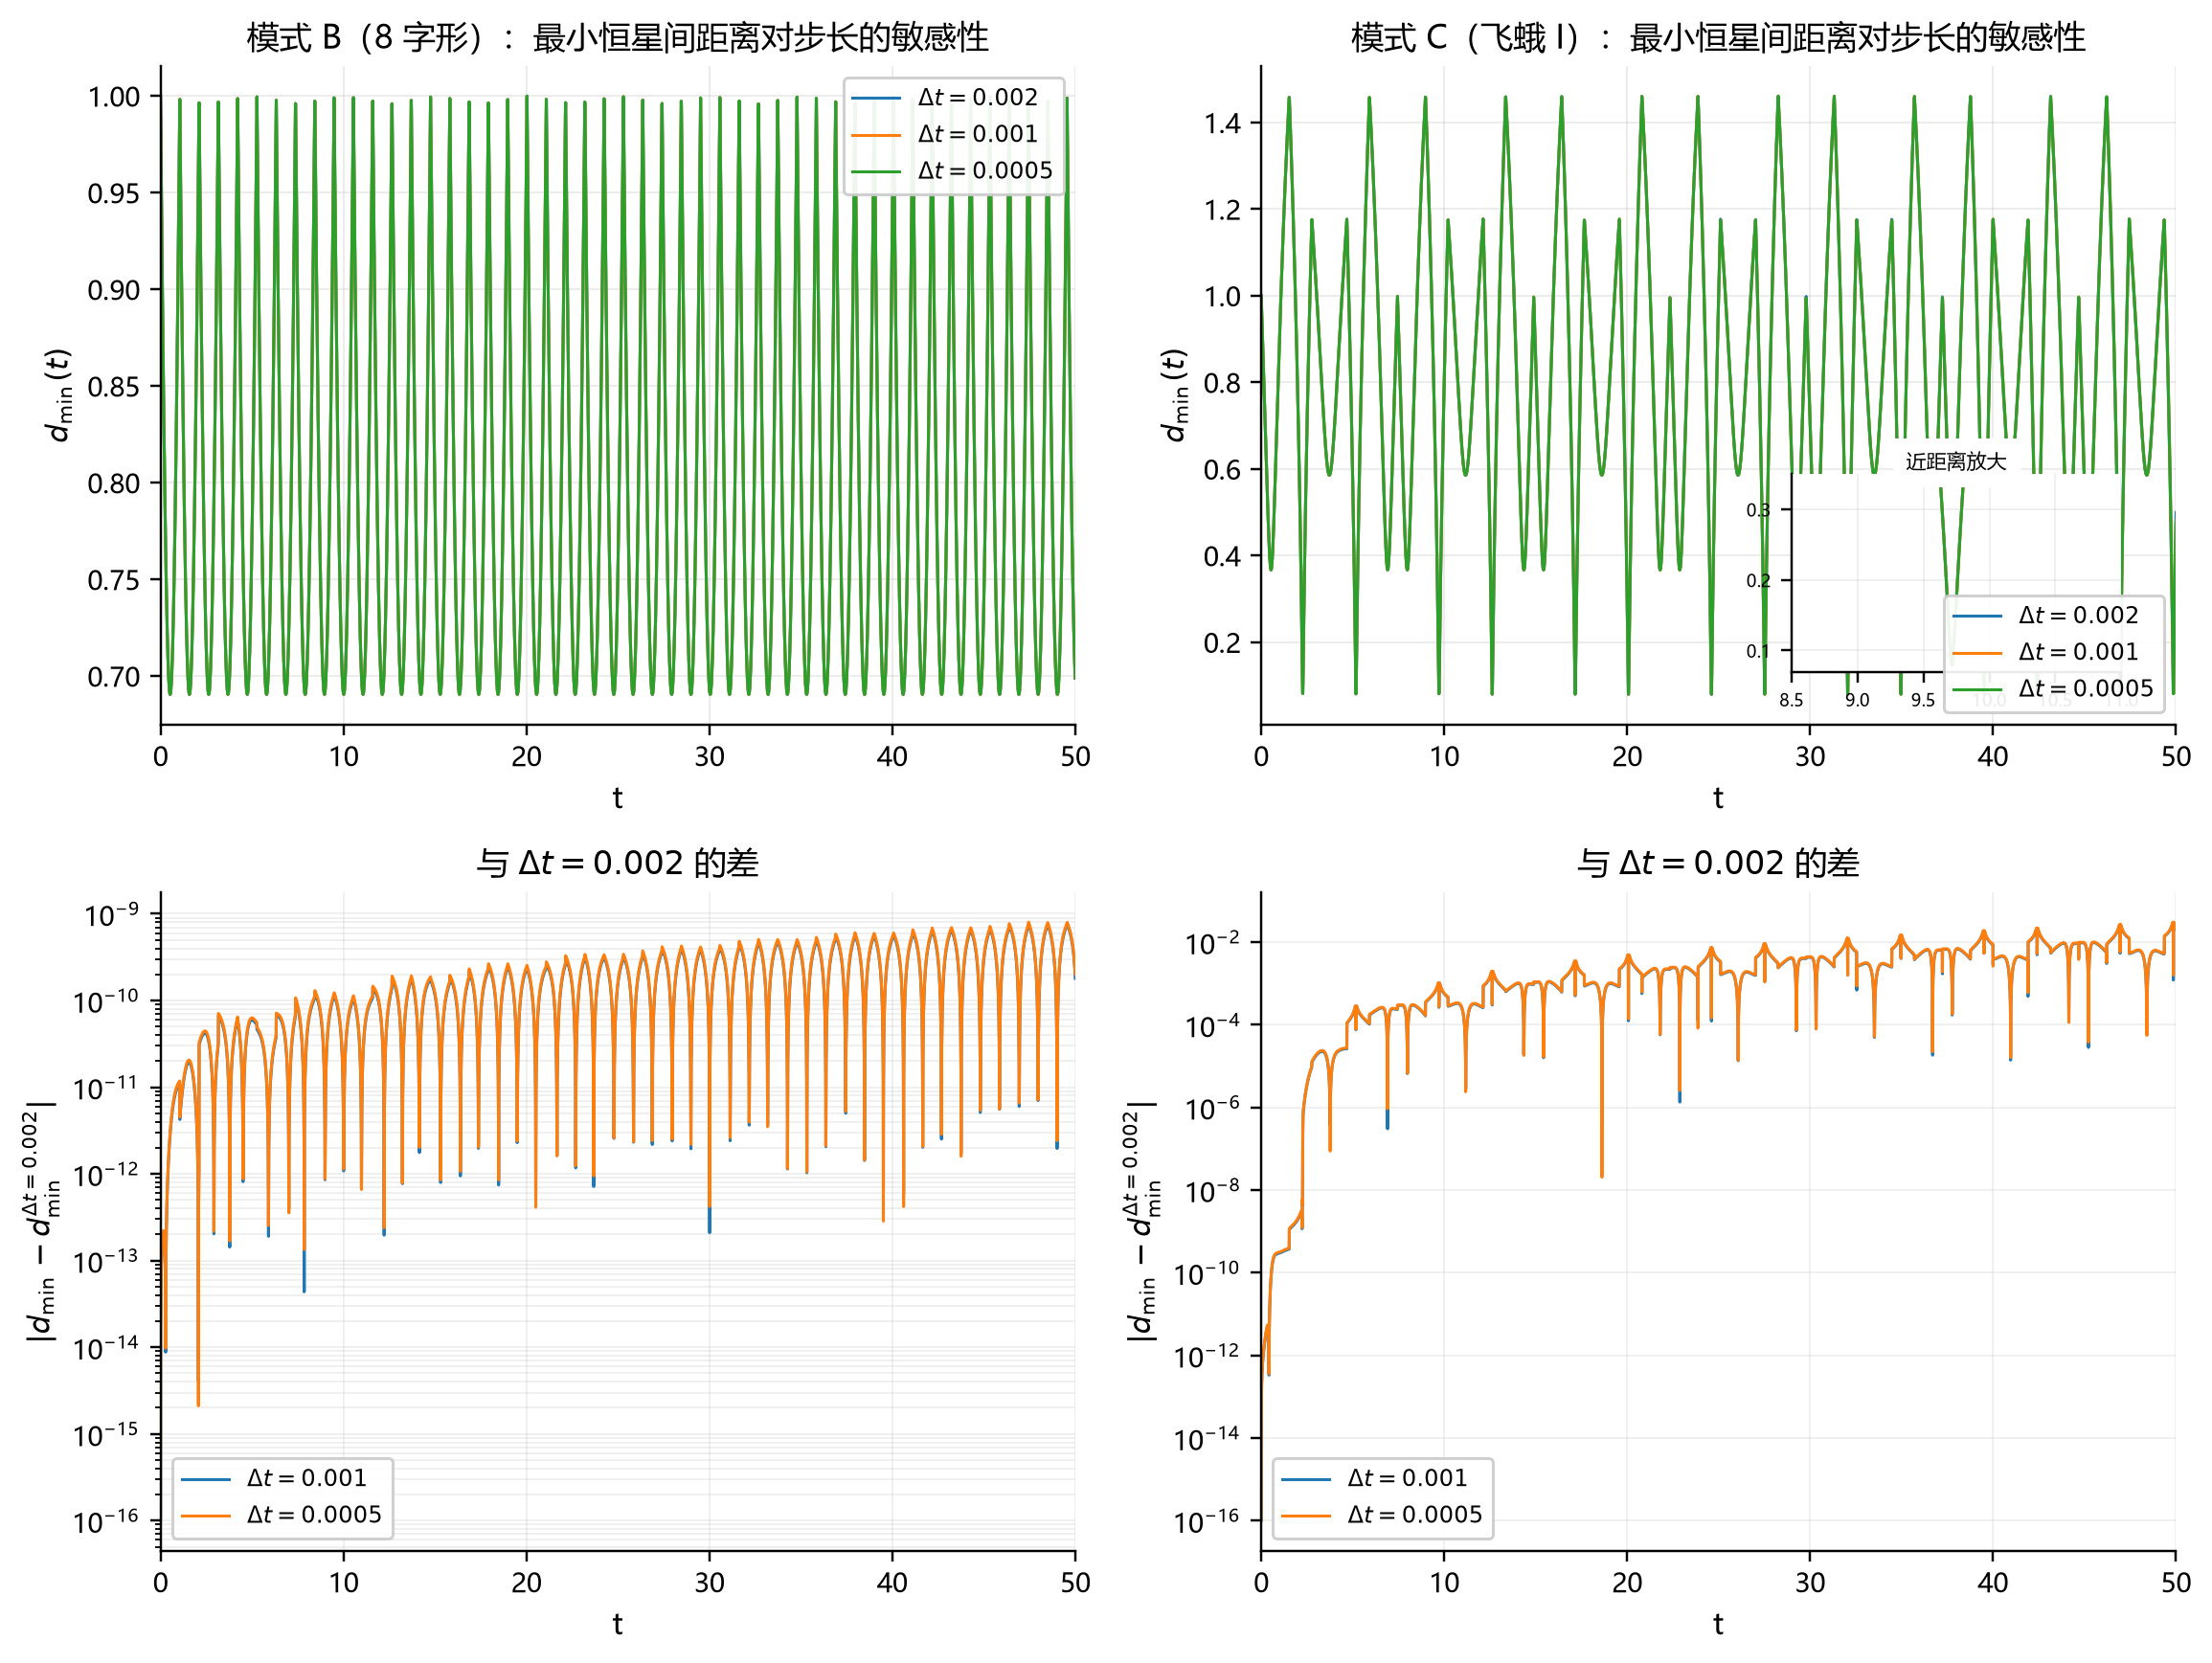
\includegraphics[width=0.95\textwidth]{fig6_distance_stepsize.png}
\caption{最小恒星间距离对步长的敏感性；插图为飞蛾模式在 $t\approx9.7$ 附近的近距离交会。}
\label{fig:stepdist}
\end{figure}

\subsection{结果与解释}
\textbf{8 字形：} 能量误差从 $\Delta t=0.002$ 的 $6.6\times10^{-12}$ 降到 $0.001$ 的
$2.0\times10^{-13}$、$0.0005$ 的 $3.1\times10^{-14}$；$d_{\min}$、$d_{\max}$ 在 6 位小数内
不变；位置差最大 $1.2\times10^{-9}$，速度差 $2.3\times10^{-9}$，$d_{\min}$ 差
$7.6\times10^{-10}$。这是一条“数值友好”的轨道：没有强近距离交会，RK4 的四阶收敛表现得很
干净，继续减小步长后误差接近双精度舍入平台（$10^{-14}$）。

\textbf{飞蛾 I：} 能量误差从 $2.46\times10^{-4}$ 降到 $7.72\times10^{-6}$、$2.42\times10^{-7}$，
相邻步长之间约缩小 32 倍；$d_{\min}$ 从 $0.079388$ 变到 $0.079422$、$0.079405$，
$d_{\max}$ 从 $2.159999$ 变到 $2.160056$、$2.160061$。但轨迹并不随步长单调收敛：
$\Delta t=0.002$ 与 $0.001$ 的最大位置差为 $0.042$，速度差可达 $1.82$，$d_{\min}$ 差
$0.029$；继续把步长减到 $0.0005$，位置差仍为 $0.043$，没有明显下降。原因不是能量不守恒，
而是飞蛾轨道在 $t\approx24.6$、$47$ 附近的近距离交会对相位极其敏感：步长改变一点，交会时刻
就移动，位置和速度在交会附近被放大，但能量仍然守恒得很好。这是“能量误差小 $\ne$ 轨迹准确”
的典型例子。

能量误差的下降倍数约为 32，接近 $2^5$。RK4 的全局误差名义上是 $O(\Delta t^4)$，但这里的
最大能量误差主要来自近距离交会附近的局部误差，局部误差按 $\Delta t^5$ 缩放；因此观测到的
比值更接近五阶局域标度，不能简单用单一阶数概括。表~\ref{tab:step} 中观测阶
$p=\log_2(\varepsilon_E(\Delta t)/\varepsilon_E(\Delta t/2))$：B 的第一个比值为 5.08，
第二个为 2.65（已受 $10^{-14}$ 舍入平台影响）；C 的两个比值均为 5.00。对 8 字形，误差已经
接近舍入平台，不能再用单一幂次拟合。

\textbf{模式 A 的教训：} 它的能量误差可以很小（RK4 $\Delta t=0.001$ 为 $3.9\times10^{-6}$），
但轨迹在 $t=30$ 时已偏离解析解 $2.09$。原因是能量守恒只约束一个标量，而不稳定模式会把微小的
相位误差指数放大。对不稳定轨道，必须同时检查能量、与解析解/高精度参考的偏差，以及不同步长/
容差下的收敛性。

\subsection{数值建议}
\begin{itemize}[leftmargin=2em,itemsep=2pt]
\item 对普通有界轨道，RK4 $\Delta t=0.001$ 已能给出 $10^{-12}$ 量级的能量误差；但不要只看
能量，要看轨迹收敛。
\item 对含近距离交会的轨道（如飞蛾 I），固定步长 RK4 的相位误差可能远大于扰动信号；本文的
扰动实验改用 DP45（$\mathrm{rtol}=10^{-13}$），并用两种容差复核。
\item 对不稳定平衡/周期轨道（如模式 A），双精度不足以维持 $t=50$；应使用解析解、更高精度
算术（约 27 位有效数字）或把有限时间缩短到误差增长可接受的范围。
\item 所有长时间积分都应监控 $d_{\min}$、$d_{\max}$ 和能量；$0.05$ 的预警阈值应作为事件检测，
而不是事后检查。
\end{itemize}

% ================= 8 稳定性综合 =================
\section{有限时间稳定性的综合讨论}\label{sec:stability}
\begin{table}[H]
\centering\footnotesize
\setlength{\tabcolsep}{3pt}
\caption{四种模式的有限时间稳定性对比}
\label{tab:stability}
\begin{tabular}{@{}lcccccc@{}}
\toprule
模式 & $0\le t\le50$ 有界 & $d_{\min}-0.05$ & 对 $10^{-4}$ 扰动 & 线性稳定性 & 结论\\
\midrule
A & 是（解析） & 0.95 & 指数增长，$t\approx15.5$ 瓦解 & $\lambda=1.2247$（线性不稳定） & 不稳定\\
B & 是 & 0.64 & $\delta\le6.3\times10^{-3}$，有界 & 已知线性稳定 & 有限时间稳定\\
C & 是 & 0.029 & $\delta\le1.2\times10^{-2}$，有界但敏感 & 未证明 & 边缘\\
D & 是 & 0.35 & $\delta\le7.6\times10^{-4}$ & 未证明；时间尺度分离 & 鲁棒\\
\bottomrule
\end{tabular}
\end{table}

模式 A 是唯一一个“未扰动严格周期、但对扰动不稳定”的例子。它的不稳定性来自等边三角形构型的
鞍点性质，而不是数值误差；数值误差只是提前触发了它。模式 B 是已知的线性稳定周期轨道，
本文的 50 时间扰动实验与之一致。模式 C 的最小距离只有 $0.079$，裕量只有 $0.029$，属于边缘
案例；模式 D 依靠时间尺度分离获得鲁棒性，但严格地说，层级三体在极长时间下仍可能出现混沌或
逃逸，本文没有证明永久稳定。

题目提醒“在 $t\le50$ 内没有失稳不等于永久稳定；未扰动轨道周期重复，也不自动意味着对扰动
稳定”。本文的四个模式正好覆盖了这句话的几种情形：A 周期但不稳定，B 周期且（有限时间）稳定，
C 有界但边缘，D 非周期但鲁棒。判断一个模式是否“稳定”，必须明确时间尺度、扰动幅度和稳定性
的定义。

% ================= 9 AI 使用 =================
\section{AI 使用记录与核验}\label{sec:ai}

本作业允许 AI 辅助编程和查找思路。本文使用 DeepSeek Harness 的编码助手（deepseek-flash）
完成以下工作：生成 RK4/DP45 积分器与绘图脚本的初稿；检索零角动量对称族的三体周期轨道初值；
帮助组织报告结构。所有数值结果均由本地程序重新计算，AI 给出的候选轨道和结论都做了独立检验。
下面记录三次具体使用及其核验过程。

\begin{table}[H]
\centering\footnotesize
\caption{AI 使用与核验记录}
\label{tab:ai}
\begin{tabular}{@{}p{4.7cm}p{5.5cm}p{4.6cm}@{}}
\toprule
AI 的输出/建议 & 核验方法 & 结果\\
\midrule
生成三体右端函数、RK4 和 DP45 积分器，并建议用解析 Lagrange 解检验。 &
手算 $t=0$ 的加速度并与 $-\omega^2\vect r$ 比较；把解析解代入方程检查残差；检查能量和动量
守恒；用两种步长比较能量误差。 &
残差 $1.1\times10^{-15}$；能量误差随步长下降；代码用于全部计算。\\
检索 Šuvakov--Dmitrašinović 的对称族初值，并推荐 butterfly I 作为“新模式”。 &
用本文积分器独立积分一个周期，检查 $0.05\le d_{ij}<10$；不直接采用文献结论。 &
butterfly I 的 $d_{\min}=0.0110<0.05$，不合格，剔除；moth I 的 $d_{\min}=0.0794$，保留。\\
建议直接用双精度数值积分把模式 A 模拟到 $t=50$，并报告“有界”。 &
与解析解逐点比较；对旋转系做线性化，求最大特征值；检查不同积分器的偏差。 &
数值解在 $t\approx30$ 偏离解析解 $O(1)$；线性 $\lambda=1.2247$，确认是物理不稳定被舍入
误差触发。改用解析解呈现模式 A，并单列数值精度实验。\\
\bottomrule
\end{tabular}
\end{table}

一个具体的“AI 错误”例子是 butterfly I：AI 只根据文献说它是已知周期轨道，但它在题目给定的
$0.05$ 阈值下最小距离只有 $0.0110$，不满足有界模式的定义。如果直接相信 AI 的推荐，就会把
一个不合格的轨道写进结果表。这说明 AI 适合提供思路和初稿，但物理判据必须由程序独立复核。

另一个例子是模式 A 的“双精度能算到 50”这一直觉。AI 最初建议直接数值积分并报告有界；但解析解
对比显示 $t\approx30$ 后偏差已达 $O(1)$，而能量误差仍只有 $10^{-6}$。进一步做线性稳定性分析
得到 $\lambda=1.2247$，才解释清楚这是物理不稳定而非程序 bug。最终报告中模式 A 的数据来自
解析解，数值积分只作为“数值精度”的反面教材。

% ================= 10 结论 =================
\section{结论}\label{sec:conclusion}
本文在 $0\le t\le50$ 内检验了四种平面等质量三体有界模式：Lagrange 等边三角形、8 字形、
飞蛾 I 和层级三体。模式 A、B 为题目给定；模式 C、D 为本文新找到/构造的模式，均给出完整
初始条件、轨迹、距离和模拟时长。四种模式都满足 $0.05\le d_{ij}<10$（A 由解析解，B/C/D 由
数值积分），其中 C、D 是新模式。

主要结论如下：
\begin{itemize}[leftmargin=2em,itemsep=2pt]
\item 模式 A 是严格周期解（$\omega=\sqrt3$，$T=3.6276$，$d\equiv1$），但线性增长率
$\lambda=1.2247$；$10^{-4}$ 扰动在 $t\approx8$ 后使三角形瓦解，$t\approx15.55$ 触发预警。
双精度数值积分也会在 $t\approx30$ 后偏离解析解，需约 27 位有效数字才能维持到 $t=50$。
\item 模式 B 的 8 字形在 50 时间内保持有界，扰动分离仅 $6.3\times10^{-3}$；与已知的线性
稳定性一致。
\item 模式 C 的飞蛾 I 最小距离 $0.0794$，扰动后有界（$\delta\le1.2\times10^{-2}$），但裕量
仅 $0.029$，属于边缘稳定。
\item 模式 D 的层级三体最小距离 $0.399$，扰动分离 $4.7\times10^{-4}$；时间尺度分离
（1.12 对 29.0）带来鲁棒性。
\item 步长检验：8 字形的 RK4 能量误差 $6.6\times10^{-12}\to3.1\times10^{-14}$；飞蛾 I 的
能量误差 $2.46\times10^{-4}\to2.42\times10^{-7}$，但近距离交会处的位置差可达 $0.042$、
$d_{\min}$ 差 $0.029$，轨迹不随步长单调收敛。扰动实验必须用高精度自适应积分，不能只用固定
步长 RK4。
\end{itemize}
最终的回答是：特殊初始条件确实可以让三颗恒星在有限时间内做有规律的运动；但“有规律”不等于
“稳定”。等边三角形是周期解却不稳定，8 字形在有限时间内稳定，飞蛾 I 处于边缘，层级三体靠
时间尺度分离获得鲁棒性。判断稳定性必须同时说明时间尺度、扰动幅度和数值精度，并区分有限时间
有界与永久稳定。

% ================= 附录 =================
\appendix
\section{程序结构与复现}\label{app:code}
本作业的全部代码和数据都在 \texttt{3body} 目录下，结构如下：
\begin{itemize}[leftmargin=2em,itemsep=1pt]
\item \texttt{three\_body.py}：物理模型、初始条件、RK4/DP45 积分器、能量/距离/分离等诊断函数。
\item \texttt{run\_experiments.py}：跑全部模式、扰动实验、步长对比和候选筛选，输出 \texttt{results/}。
\item \texttt{make\_figures.py}：从 \texttt{results/} 生成 \texttt{figures/} 下的 7 张图。
\item \texttt{make\_report.py}：生成 DOCX 版报告（本 PDF 由 \texttt{latex/} 中的 \LaTeX{} 源码编译）。
\item \texttt{test\_three\_body.py}：8 个断言测试（力平衡、能量守恒、解析解、扰动质心等）。
\item \texttt{results/}：\texttt{trajectories.npz}、\texttt{summary.json}、\texttt{summary.csv}、
\texttt{screening.csv}。
\end{itemize}
复现命令（Windows，Python 3.12+）：
\begin{lstlisting}[language=bash,numbers=none]
python run_experiments.py
python make_figures.py
python test_three_body.py
\end{lstlisting}
依赖：numpy、matplotlib、python-docx；测试脚本无需 pytest。所有随机性均无（初值固定），结果
对平台差异只会有 $10^{-12}$ 量级的数值差别。

下面是核心代码片段（完整代码见 \texttt{three\_body.py}）：
\begin{lstlisting}
def accelerations(pos):
    """pos shape (3,2); return a_i = sum_j (r_j-r_i)/|r_j-r_i|^3."""
    diff = pos[None, :, :] - pos[:, None, :]   # diff[i,j] = r_j - r_i
    r2 = np.einsum("ijk,ijk->ij", diff, diff)
    np.fill_diagonal(r2, np.inf)
    inv_r3 = r2 ** (-1.5)
    return np.einsum("ij,ijk->ik", inv_r3, diff)

def rhs(state):
    out = np.empty_like(state)
    out[:, :2] = state[:, 2:]
    out[:, 2:] = accelerations(state[:, :2])
    return out
\end{lstlisting}

近距离停止逻辑：
\begin{lstlisting}
d = pair_distances(state[:, :2])
if np.min(d) < 0.05:
    stop_reason = "close_encounter"
    stop_time = t
    break
\end{lstlisting}

% ================= 参考文献 =================
\section*{参考文献}
\addcontentsline{toc}{section}{参考文献}
\begin{enumerate}[label={[\arabic*]},leftmargin=2.2em,itemsep=1pt]
\item Chenciner A., Montgomery R. A remarkable periodic solution of the three-body problem in
the case of equal masses. \emph{Annals of Mathematics}, 2000, 152(3): 881--901.
\item Šuvakov M., Dmitrašinović V. Three classes of Newtonian three-body planar periodic orbits.
\emph{Physical Review Letters}, 2013, 110: 114301. arXiv:1303.0181.
\item Sim\'o C. Dynamical analysis of the Chenciner--Montgomery orbit. In:
\emph{Hamiltonian Systems and Celestial Mechanics}, 2002.
\item Hairer E., Nørsett S. P., Wanner G. \emph{Solving Ordinary Differential Equations I}.
Springer, 1993.（Dormand--Prince 5(4) 方法）
\item Giordano N. J., Nakanishi H. \emph{Computational Physics}. 2nd ed. Pearson, 2006.
\item NEMO data file: planar 3body initial conditions [Šuvakov \& Dmitrašinović (2013)].
\url{https://gitlab.astro.rug.nl/teuben/nemo/-/blob/master/data/3body.tab}
\end{enumerate}

\end{document}
